%% main.tex — ODeSSy / Super-Analysis — CGO 2027 R2 submission draft
%% Build: pdflatex main && bibtex main && pdflatex main && pdflatex main
%% Numbers sourced from docs/PAPER_FACTS.md v4-final (Aug 18 2026).
%% Figures expected in the project root: spectrum.png, super-opt_cost.png,
%% super-analysis_cost.png, smt_latencies.png  (PNG for the draft; convert
%% to PDF for camera-ready).
%%
\begin{filecontents*}[overwrite]{odessy.bib}
@inproceedings{serebryany2012asan,
  author = {Konstantin Serebryany and Derek Bruening and Alexander Potapenko and Dmitriy Vyukov},
  title = {{AddressSanitizer}: A Fast Address Sanity Checker},
  booktitle = {USENIX ATC},
  year = {2012}
}
@inproceedings{sasnauskas2017souper,
  author = {Raimondas Sasnauskas and Yang Chen and Peter Collingbourne and Jeroen Ketema and Gratian Lup and Jubi Taneja and John Regehr},
  title = {Souper: A Synthesizing Superoptimizer},
  booktitle = {arXiv:1711.04422},
  year = {2017}
}
@inproceedings{schkufza2013stoke,
  author = {Eric Schkufza and Rahul Sharma and Alex Aiken},
  title = {Stochastic Superoptimization},
  booktitle = {ASPLOS},
  year = {2013}
}
@inproceedings{massalin1987superoptimizer,
  author = {Henry Massalin},
  title = {Superoptimizer: A Look at the Smallest Program},
  booktitle = {ASPLOS},
  year = {1987}
}
@inproceedings{tate2009equality,
  author = {Ross Tate and Michael Stepp and Zachary Tatlock and Sorin Lerner},
  title = {Equality Saturation: A New Approach to Optimization},
  booktitle = {POPL},
  year = {2009}
}
@inproceedings{demoura2008z3,
  author = {Leonardo de Moura and Nikolaj Bj{\o}rner},
  title = {{Z3}: An Efficient {SMT} Solver},
  booktitle = {TACAS},
  year = {2008}
}
@inproceedings{lattner2004llvm,
  author = {Chris Lattner and Vikram Adve},
  title = {{LLVM}: A Compilation Framework for Lifelong Program Analysis \& Transformation},
  booktitle = {CGO},
  year = {2004}
}
@inproceedings{lopes2021alive2,
  author = {Nuno P. Lopes and Juneyoung Lee and Chung-Kil Hur and Zhengyang Liu and John Regehr},
  title = {Alive2: Bounded Translation Validation for {LLVM}},
  booktitle = {PLDI},
  year = {2021}
}
@inproceedings{grosser2012polly,
  author = {Tobias Grosser and Armin Gr{\"o}{\ss}linger and Christian Lengauer},
  title = {Polly: Performing Polyhedral Optimizations on a Low-Level Intermediate Representation},
  booktitle = {Parallel Processing Letters},
  year = {2012}
}
@inproceedings{relaxingalias2025,
  author = {Anonymous},
  title = {Relaxing Alias Analysis: Exploring the Unexplored Space},
  booktitle = {PLDI},
  year = {2025},
  note = {Citation to be completed}
}
@inproceedings{taneja2020knownbits,
  author = {Jubi Taneja and Zhengyang Liu and John Regehr},
  title = {Testing Static Analyses for Precision and Soundness},
  booktitle = {CGO},
  year = {2020}
}
@article{reynolds2002separation,
  author = {John C. Reynolds},
  title = {Separation Logic: A Logic for Shared Mutable Data Structures},
  journal = {LICS},
  year = {2002}
}
@inproceedings{leino2010dafny,
  author = {K. Rustan M. Leino},
  title = {Dafny: An Automatic Program Verifier for Functional Correctness},
  booktitle = {LPAR},
  year = {2010}
}
@misc{ubsanDocs,
  author = {{LLVM Project}},
  title = {UndefinedBehaviorSanitizer Documentation},
  howpublished = {\url{https://clang.llvm.org/docs/UndefinedBehaviorSanitizer.html}},
  year = {2026}
}
@misc{cloudlab,
  author = {Dmitry Duplyakin and others},
  title = {The Design and Operation of {CloudLab}},
  howpublished = {USENIX ATC},
  year = {2019}
}
\end{filecontents*}
%%
\documentclass[sigplan,screen,review,anonymous]{acmart}
\AtBeginDocument{\providecommand\BibTeX{{Bib\TeX}}}
%% Rights placeholders — ACM supplies real values at camera-ready. Do not edit.
\setcopyright{acmlicensed}
\copyrightyear{2027}
\acmYear{2027}
\acmDOI{XXXXXXX.XXXXXXX}
\acmConference[CGO '27]{IEEE/ACM International Symposium on Code Generation and Optimization}{March 20--24, 2027}{TBD}
\acmISBN{978-1-4503-XXXX-X/27/03}
%%\acmSubmissionID{XXX}
%% Code listings for the worked examples
\usepackage{listings}
\usepackage{algorithm}
\usepackage{algpseudocode}
\definecolor{codecomment}{gray}{0.45}
\definecolor{codekw}{RGB}{0,90,160}
\definecolor{trapred}{RGB}{200,20,20}
\lstdefinestyle{odessy}{
  basicstyle=\small\ttfamily,
  keywordstyle=\color{codekw}\bfseries,
  commentstyle=\color{codecomment}\itshape,
  columns=fullflexible,
  keepspaces=true,
  breaklines=false,
  xleftmargin=0.5em
}
%% Convenience macros
\newcommand{\odessy}{ODeSSy}
\newcommand{\tool}{\odessy}
\newcommand{\pct}[1]{#1\%}
\newcommand{\den}[1]{[\![#1]\!]}
\newcommand{\FIGURE}[1]{\begin{center}\fbox{\parbox{0.9\linewidth}{\centering\vspace{2em}\textit{[Figure placeholder: #1]}\vspace{2em}}}\end{center}}
\begin{document}
\title[Super-Analysis for Compiler Optimization]{Super-Analysis for Aggressive yet Scalable Compiler Optimization}
\author{Anonymous Author(s)}
\affiliation{\institution{Anonymous Institution}\city{City}\country{Country}}
\email{anonymous@example.com}
\renewcommand{\shortauthors}{Anon. et al.}
\begin{abstract}
Aggressive compiler optimization today occupies two distant extremes.
Conventional optimizers run in milliseconds but reason through ad-hoc
heuristics that miss opportunities; superoptimizers synthesize faster code
but take hours, confining them to small kernels and offline use. We introduce
\emph{super-analysis}, a middle ground that uses an SMT solver purely for
\emph{analysis} while transformations remain conventional, avoiding
synthesis entirely. The key argument for super-analysis is that many simple, yet fruitful transformations require complex reasoning: proving a safety check dead often needs facts from four
independent LLVM analyses \emph{simultaneously} --- a conjunctive entailment
problem suited to a solver, not to any single dataflow pass.
We instantiate
super-analysis in \tool{}, an LLVM pass that proves sanitizer traps and
native-language safety checks unreachable and deletes them.
One mechanism serves three frontends and yields speedups in each:
\tool{} generates code up to $4.16\times$ faster than LLVM -O3 for a GEMM implemented in Julia, speeds up a Swift SHA-256 kernel by \pct{8.8}, and delivers a
whole-library runtime win of \pct{2.6} for zstd compression in C. Latency
is controllable:
\pct{96} of proofs survive a 100\,ms per-query SMT timeout budget, making
super-analysis viable as an online compiler pass rather than an offline
tool.
\end{abstract}
\begin{CCSXML}
<ccs2012>
 <concept>
  <concept_id>10011007.10011006.10011041.10011048</concept_id>
  <concept_desc>Software and its engineering~Runtime environments</concept_desc>
  <concept_significance>100</concept_significance>
 </concept>
 <concept>
  <concept_id>10011007.10011006.10011041</concept_id>
  <concept_desc>Software and its engineering~Compilers</concept_desc>
  <concept_significance>500</concept_significance>
 </concept>
 <concept>
  <concept_id>10003752.10003790.10011740</concept_id>
  <concept_desc>Theory of computation~Automated reasoning</concept_desc>
  <concept_significance>300</concept_significance>
 </concept>
</ccs2012>
\end{CCSXML}
\ccsdesc[500]{Software and its engineering~Compilers}
\ccsdesc[300]{Theory of computation~Automated reasoning}
\keywords{SMT solvers, compiler optimization, sanitizers, bounds-check
elimination, undefined behavior, LLVM}
\maketitle
%% =====================================================================
\section{Introduction}
\label{sec:intro}
Compiler optimization research today occupies two distant extremes of a
cost--precision spectrum. At one end, conventional optimizers such as
LLVM's O3 pipeline~\cite{lattner2004llvm} make millions of decisions in
milliseconds, each justified by an ad-hoc heuristic or a lightweight
dataflow analysis; the heuristics are fast precisely because each one
reasons locally and gives up early. At the
other end, superoptimizers~\cite{massalin1987superoptimizer,
schkufza2013stoke, sasnauskas2017souper} hand the entire problem ---
analysis \emph{and} transformation --- to an expensive decision procedure
that aggressively searches for replacement code, achieving precision that heuristics
cannot match at costs that confine them to peephole windows and offline
runs.
\begin{figure}[t]
\centering
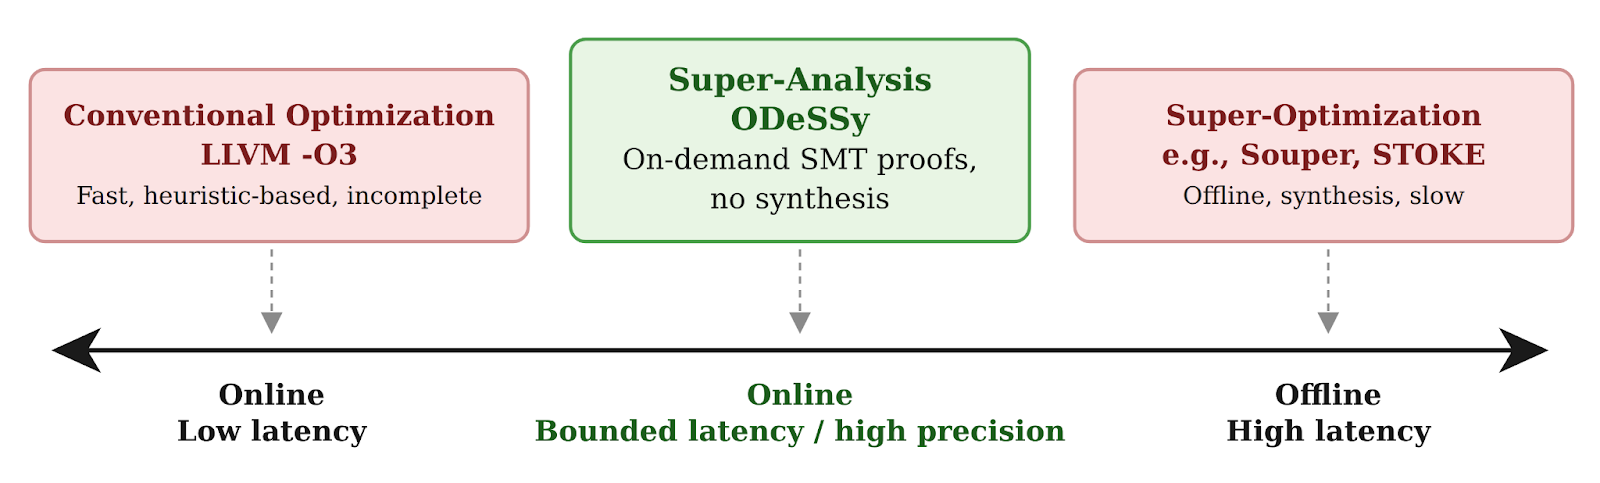
\includegraphics[width=\linewidth]{spectrum.png}
\caption{The cost--precision spectrum of aggressive compiler
optimization. Conventional pipelines are online but heuristic and
incomplete; superoptimizers are precise but offline. Super-analysis
occupies the unpopulated middle: on-demand SMT proofs at bounded latency,
with no synthesis, inside the compilation pipeline.}
\Description{A horizontal axis from online/low-latency on the left to
offline/high-latency on the right. Three boxes sit along it: Conventional
Optimization (LLVM -O3) on the left, Super-Analysis (ODeSSy) in the
middle, and Superoptimization (Souper, STOKE) on the right.}
\label{fig:spectrum}
\end{figure}
This paper argues for a middle ground we call \emph{super-analysis}
(Figure~\ref{fig:spectrum}): use
the decision procedure for \emph{analysis only}, and leave transformation
to the conventional machinery that already exists. No code is synthesized;
no search is performed. The solver answers exactly one kind of question
--- \emph{is this program point reachable under this context?} --- and a
standard, trivially correct transformation (deleting an unreachable branch)
consumes the answer.
We use an SMT solver as an analysis oracle and feed it with the encoded formula $Context \land Query$ and ask if it is satisfiable. Soundness is preserved by construction: an
\textsc{unsat} verdict is a proof, a \textsc{sat} or \textsc{unknown}
verdict changes nothing.
Why should a solver find opportunities that forty years of heuristics
miss? Our central empirical finding is that the missed opportunities are
typically not hard to \emph{transform} but hard to \emph{justify}. Proving
one bounds check dead in a real SHA-256 kernel requires the return-value
range of one function, a scalar-evolution loop bound, a value-range fact
on a third value, and two dominating branch conditions ---
\emph{simultaneously}. Each fact lives in a different LLVM analysis; no
single pass computes their conjunction, and the phase-ordering problem
ensures no fixed pipeline ever will. Deciding satisfiability of a
complex conjunction is, on principle, an entailment
problem --- exactly what an SMT solver decides and exactly what a
heuristic cannot. Our tool extracts the unsat core of every proof, so this
claim is not an intuition but a measurement: the cores name the
contributing analyses, and the majority of our nontrivial proofs draw on
two to four sources at once (\S\ref{sec:results-static}).
We instantiate super-analysis in \tool{}\footnote{On-Demand SMT System.},
an LLVM module pass targeting one of the most consequential class of
provably-dead code in modern software: \emph{safety checks}. Sanitizers
such as UBSan~\cite{ubsanDocs} and the native checks of memory-safe
languages (Swift bounds and overflow checks, Rust panics, Julia bounds
errors) compile to trap-guarded branches whose hot-path cost is the
standing tax of memory safety --- we measure it at up to \pct{9.0} on
the fully sanitized zstd library and up to $4$--$5\times$ on native-language kernels (Swift, Julia implementations of nbody, GEMM, respectively).
Today the only recourse on hot paths is to turn checks \emph{off}
wholesale (\texttt{-Ounchecked}, \texttt{--check-bounds=no}), trading away
the safety guarantee entirely. \tool{} offers the sound alternative:
delete exactly the checks that are provably redundant with the guards,
contracts, and invariants already present in the program, and keep every
check that is not --- each deletion certified by an unsat core, audited
for vacuity, and validated by byte-identical program output.
\tool{} is sandwiched between two LLVM -O3 runs in our pipeline. The first -O3 run injects the sanitizers and performs intial optimizations. \tool{} then eliminated many of the injected traps and sanitizers, followed by the second -O3 run that cleans the IR and performs new transformations enabled by \tool{}. \tool{} eliminates up to \pct{35.0} sanitizers left by a single -O3 run in large scale C repositories, and up to \pct{13.6} of sanitizers left after 2 consecutive -O3 runs. In our experiments we compare \tool{} against $2\times$-O3.
Super-analysis is a general compilation paradigm rather than a single
optimization, and it carries one open problem we deliberately defer:
\emph{when is expensive analysis worth invoking?} A solver consulted
indiscriminately at every program point would be ruinous, and deciding
where precision repays its cost demands a cost model no compiler has.
Safety-check elimination is the ideal first instantiation precisely
because it answers that question for free. The work list is given --- run
exactly where the traps are, a set the frontend already enumerates. The
payoff needs no cost model --- erasing a check simplifies the program control-flow, allowing other optimizations to be performed on by subsequent passes. This
application therefore isolates the paradigm's contribution --- precision
of analysis --- from the question it defers, and we return in
\S\ref{sec:future} to what invoking super-analysis elsewhere would
require.
This paper makes the following contributions:
\begin{itemize}
\item \textbf{Super-analysis} (\S\ref{sec:superanalysis}): an aggressive compilation paradigm
  positioning between conventional heuristic-based optimization and superoptimization. The general recipe for this paradigm is to use solvers (SMT in particular) as an analysis oracle, while applying cheap conventional rules-based transformation for optimization.
\item \textbf{\tool{}} (\S\ref{sec:system}): a three-stage LLVM pass
  (serial discovery, parallel solve, serial transform) that eliminates sanitizer checks and optimizes the resulting IR. ODeSSy supports C/C++, Swift, and Julia as frontends and can enable hot-path transformations and speedups.
\item \textbf{An honest evaluation} (\S\ref{sec:results}):
  \tool{} removes up to \pct{13.6} of checks on real repositories.
  Runtime experiments with 30-repetition medians on two target architectures (x86 and M-series) show \emph{when} elimination pays: removing hot-loop checks has a cascading effect, unlocking further transformations (unrolling, vectorization, etc) that enables up to $4.16\times$ speedups for some widely used kernels.
\item \textbf{Flexible Compiler Latency} (\S\ref{sec:results-cost}): \tool{} proofs are generally cheap: \pct{96} of
  zlib's proofs survive a 100\,ms per-query budget. By multi-threading and strict SMT timout budgets \tool{} can compile up to $4.8\times$ faster, making it an online compiler.
\end{itemize}
%% =====================================================================
\section{Background and Related Work}
\label{sec:related}
\paragraph{Superoptimization.} A superoptimizer tries to search a large space of programs for a faster or shorter alternative to the initial code.
Massalin's original superoptimizer~\cite{massalin1987superoptimizer}
enumerated every instruction sequence up to a length bound and kept the
shortest one that matched the target on test inputs. Two lines of work
made the idea provably sound and practical. STOKE~\cite{schkufza2013stoke} replaces
enumeration with stochastic search: a Markov-chain Monte Carlo walk
mutates x86-64 kernels, scores each candidate by test-case correctness
and estimated latency, and hands the survivors to an SMT solver for a
formal equivalence proof, at costs of hours per loop-free kernel.
Souper~\cite{sasnauskas2017souper} works at the LLVM IR level: it
synthesizes replacements for bounded peephole windows and verifies each
candidate with an SMT solver. Souper is the closest relative to this
work --- same IR and solver --- and the difference is architectural.
In every superoptimizer the search proposes code and the solver
verifies it, so the solver is invoked \emph{per candidate}. \tool{}
performs no synthesis at all: its solver decides reachability over
arbitrarily structured acyclic slices, once per check site, and the
compiler's own machinery performs the rewrite. This is why
super-analysis scales to whole libraries (156k-line IR modules; 12{,}798
checks in zstd) that no synthesizing tool can process. Equality
saturation~\cite{tate2009equality} searches the same kind of space by a
different route: rather than synthesizing candidates it saturates an
e-graph with the combinations of a fixed rewrite-rule set and extracts
the cheapest result, so its search ranges over rules rather than over
arbitrary programs and no candidate needs a proof of its own.
\S\ref{sec:design-space} places these paradigms on a common map.
\paragraph{Solver-aided compilation and validation.}
Alive2~\cite{lopes2021alive2} uses SMT to prove that the code LLVM
emits behaves like the code LLVM was given, acting as a compiler
validator; \tool{} inverts the direction, using SMT to \emph{enable}
transformations the pipeline could not itself justify.
Closest in spirit to our work is Taneja et al.~\cite{taneja2020knownbits},
who use an SMT solver to test LLVM's dataflow analyses. For each expression they compute the
\emph{most precise} answer an analysis could possibly give --- the
exact set of known bits, the tightest integer range --- and compare it
with LLVM's. LLVM's answers are sound but often imprecise: only \pct{48.7} of its integer ranges and
\pct{35.0} of its demanded-bits results are as tight as possible. Two of
their findings bear on super-analysis. First, their solver-based analysis
is slow --- 9\,s per expression for known bits, 16\,s for integer
ranges --- and they conclude it is ``too slow to use at compile time.''
The cost comes from the question they ask. Finding the best abstract
value is a \emph{search} over the abstract domain: known bits takes
$2n$ solver queries for an $n$-bit value, and ranges take a binary
search, so one answer costs dozens of queries. \tool{} asks a different
and much cheaper question: one yes/no reachability query per check
site (decision rather than search), which is why our median query
takes milliseconds (\S\ref{sec:results-cost}). Second, when they compiled
four programs with the maximally precise analyses installed, three moved
by a few percent at most; the one clear win (\pct{8}--\pct{22} on bzip2)
came not from the middle-end, whose optimized IR showed only minor
differences, but from the backend, whose instruction selection consumes
known bits. We read this as support for our thesis. Sharpening
\emph{one} analysis in isolation moves the optimizer little, because
what the pipeline lacks is not better facts but the ability to
\emph{conjoin} the facts it already has across analyses; our unsat cores
measure exactly that --- the nontrivial proofs draw on two to four fact
sources at once (\S\ref{sec:conjunction}). \tool{} imports LLVM's own
imprecise results as solver premises
(\S\ref{sec:system-facts}) and leaves the conjunction to the solver.
\paragraph{Sanitizers, native checks, and check elimination.}
Safety checks are the target we chose to instantiate super-analysis on,
and they come from two sources. Sanitizers instrument C/C++ with checks
for undefined or suspicious behavior --- signed overflow, shifts, array
bounds~\cite{serebryany2012asan, ubsanDocs}; compiled with
\texttt{-fsanitize-trap}, each check lowers to a compare, a branch, and
a trapping instruction. Memory-safe languages insert equivalent checks
natively: Swift traps on overflow and out-of-bounds access by default,
Julia bounds-checks array accesses under its JIT. In both worlds the
checks are semantically identical IR patterns --- a conditional branch
to a diverging block --- which is what lets one tool serve every
frontend (\S\ref{sec:system}).
%% =====================================================================
\section{Super-Analysis}
\label{sec:superanalysis}
\begin{figure}[t]
\centering
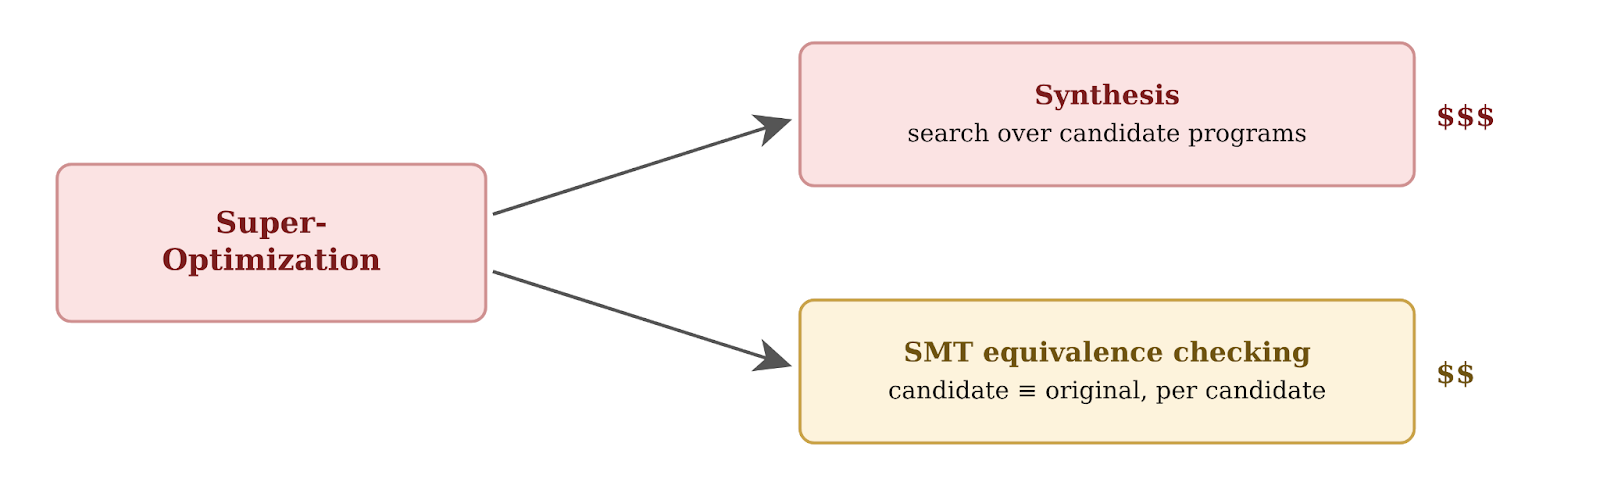
\includegraphics[width=\linewidth]{super-opt_cost.png}\\[0.9em]
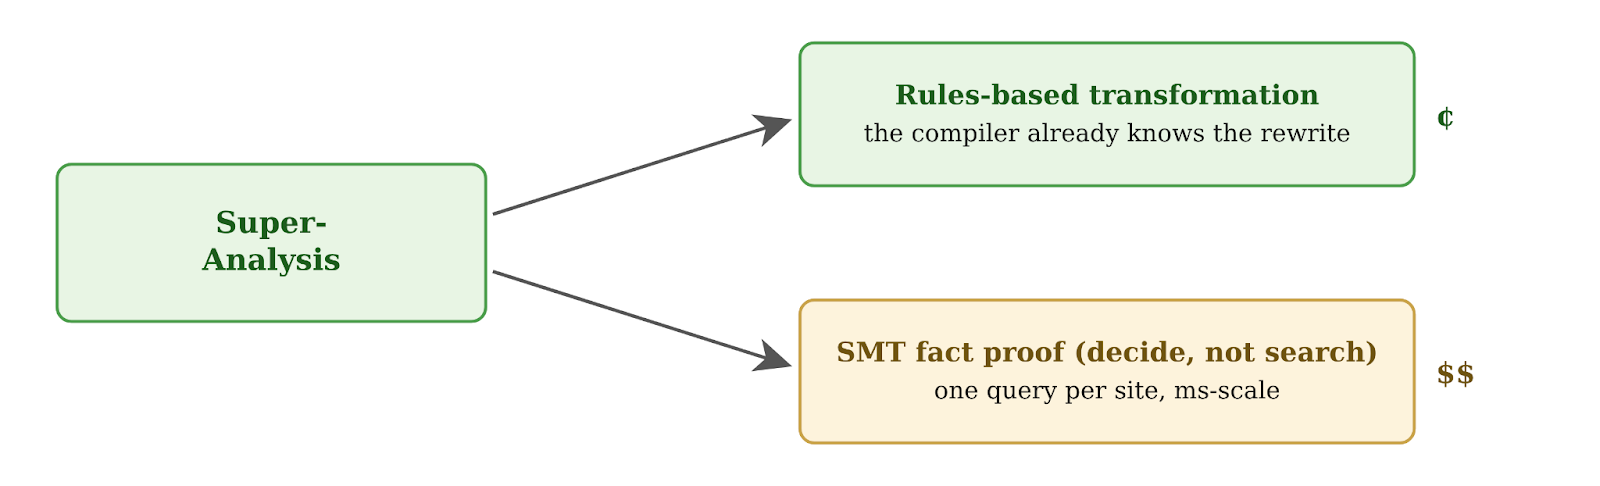
\includegraphics[width=\linewidth]{super-analysis_cost.png}
\caption{Where the cost goes. \emph{Top:} superoptimization pays twice
--- an expensive search over candidate programs, plus an SMT equivalence
check \emph{per candidate}. \emph{Bottom:} super-analysis drops the search
entirely; the transformation is a rewrite the compiler already knows, and
the solver decides one fact per site rather than validating a stream of
guesses. \textbf{Superoptimization is super-expensive because of synthesis;
super-analysis is merely expensive.}}
\Description{Two stacked flow diagrams. The top diagram shows
Superoptimization branching into Synthesis (marked triple-dollar) and SMT
equivalence checking (double-dollar). The bottom diagram shows
Super-Analysis branching into rules-based transformation (marked one cent)
and SMT fact proof (double-dollar).}
\label{fig:cost}
\end{figure}
\subsection{The design space}
\label{sec:design-space}
\begin{figure}[t]
\centering
\includegraphics[width=\linewidth]{quadrants.pdf}
\caption{Which component pays for precision. Every optimizer is an
analysis that licenses a rewrite plus a transformation that performs it,
and each can be cheap or expensive. Conventional optimization keeps both
cheap; superoptimization makes both expensive. Super-analysis takes one
asymmetric corner (a solver licenses each rewrite; the compiler applies
it). Super-transformation takes the other: exhaustive search over
combinations of rewrites whose soundness was established once, offline.
Superoptimization is the conjunction of the two. Both asymmetric corners
are under-explored; this paper develops the first.}
\Description{A two-by-two matrix. Columns: transformation cost, cheap
versus expensive. Rows: analysis cost, cheap versus expensive. Cheap/cheap
is Conventional Optimization (LLVM -O3). Cheap analysis with expensive
transformation is Super-Transformation (e.g., equality saturation), marked
under-explored. Expensive analysis with cheap transformation is
Super-Analysis (ODeSSy). Expensive/expensive is Superoptimization (Souper,
STOKE).}
\label{fig:quadrants}
\end{figure}
Conventional optimization and superoptimization differ in \emph{which
component} pays for precision. Every optimizer is two things: an
\emph{analysis} that establishes the facts licensing a rewrite, and a
\emph{transformation} that produces the replacement code. Either can be
cheap or expensive, which gives the four-way design space of
Figure~\ref{fig:quadrants}. A conventional pass has cheap analysis and
cheap transformation, and both are heuristic. A superoptimizer makes both
expensive: the search proposes code, the solver verifies it. Super-analysis
splits the difference asymmetrically: expensive, precise, \emph{sound}
analysis; cheap, conventional, trivially correct transformation. The
design wagers that in mature pipelines the transformations are not the
bottleneck --- LLVM already knows how to fold a branch, unroll a loop, and
vectorize a body --- and that what is missing is the \emph{license} to do
so.
\paragraph{The other asymmetric corner.}
The remaining cell --- cheap analysis, expensive transformation --- is
the mirror image of super-analysis, and we call it
\emph{super-transformation}: an exhaustive search for alternative code.
Synthesis, as practiced by superoptimizers, is its most aggressive form,
because the candidates are arbitrary programs. Equality
saturation~\cite{tate2009equality} is its disciplined form: it exhausts
the sequences and combinations of a fixed set of rewrite rules, which is
still an exhaustive search for replacement code, but over a space every
point of which is correct by construction. That is what keeps equality
saturation in the cheap-analysis row. Each rule is an equality proven
sound once, offline, so no candidate requires a proof of its own at
compile time. The expense is entirely on the transformation side: saturating
the e-graph and then extracting the cheapest term from it, which the
original work posed to a pseudo-boolean solver and later systems solve
greedily or with ILP. Synthesis lands in the superoptimization cell
precisely because it lacks this guarantee: an arbitrary candidate carries
no proof, so each one must be verified, and the analysis becomes
expensive as well.
The matrix therefore states the thesis of this paper exactly.
Superoptimization is super-analysis \emph{plus} super-transformation; we
take the first half and leave the second to the compiler's existing
rules. Both asymmetric corners are under-explored relative to the two
diagonal ones, and both are sound: the top row inherits soundness from
its rules, the bottom row from a per-site or per-candidate proof.
Super-analysis is the only cell that obtains a \emph{new} semantic fact
at compile time without paying for a search.
Figure~\ref{fig:cost} makes the cost consequence concrete. A
superoptimizer's dominant expense is not the solver but the
\emph{synthesis loop} that feeds it: a search over candidate programs,
each candidate requiring its own equivalence query. Super-analysis deletes
that outer loop. What remains is one decision procedure invocation per
check site --- a decision, not a search --- and a transformation the
compiler performs for free. This is why the two paradigms differ by orders
of magnitude in latency while sharing the same underlying technology, and
why super-analysis can run inside the pipeline rather than beside it
(\S\ref{sec:results-cost}).
\subsection{Encoding program context}
\label{sec:encoding}
A super-analyzer decides a property of a single \emph{program point} ---
here, whether a trap is reachable. But the property is never decided by
the point itself; it is decided by the \emph{context} that leads there.
The core machinery of the paradigm is therefore a translation: render
the context of a program point as a logical formula, and ask the solver
whether the property is consistent with it.

The translation proceeds \emph{backwards} from the point of interest.
Starting at the trap condition, it walks the chain of definitions that
feed it and the branch conditions that dominate it, and renders each
instruction as an exact equation over bit-vectors --- arithmetic,
comparisons, shifts, overflow intrinsics, and the control flow
connecting them. The resulting formula is satisfiable exactly by the
machine states that can reach the point, so reachability becomes one
satisfiability query: $\mathit{context} \wedge \mathit{trap}$.

A backward encoding cannot descend forever. It stops at
\emph{boundaries} --- loop-carried values, function calls, loads:
boxes whose interior it does not open. What crosses a boundary is a
\emph{post-condition}: a fact true of the box's result in every
execution. The weakest post-condition is no constraint at all --- the
value is a free variable --- and this is the soundness floor: anything
not understood is over-approximated, so an \textsc{unsat} verdict holds
for every concrete behavior of the unencoded parts. From that floor,
post-condition derivation is a precision dial that can in principle be
turned arbitrarily far: a range, an algebraic relation among boundary
values, a loop invariant, a full summary. Every notch is sound so long
as the stated fact holds of all executions, and every notch kills
countermodels that the floor admits.

This encoded context is the dominant machinery of super-analysis: by
proof count, most eliminations in this paper are discharged by the
translated context alone (the \emph{light} tier of
\S\ref{sec:system-facts}). What remains is the boxes the encoding
leaves closed --- which post-conditions to import for them, and why
composing those facts requires a solver.
\subsection{Why conjunction necessitates a solver}
\label{sec:conjunction}
\begin{figure*}
\begin{minipage}[t]{0.46\textwidth}
\begin{lstlisting}[style=odessy,
    morekeywords={var,for,in,let,if},
    comment={[l]{//}},
    moredelim={[is][\color{trapred}\bfseries]{|}{|}}]
var w = [UInt32](repeating: 0, count: 64)
for t in 16..<64 {
  // s0, s1: rotate-xors of w[t-15], w[t-2]
  |// implicit check (injected by compiler)|
  |if t-16 >= w.count { trap() }|
  w[t] = w[t-16] + s0 + w[t-7] + s1
}
\end{lstlisting}
\end{minipage}\hfill
\begin{minipage}[t]{0.50\textwidth}
\begin{lstlisting}[style=odessy,
    morekeywords={load,add,icmp,uge,br,label,call,void,i8,i64,i1,ptr},
    comment={[l]{;}},
    moredelim={[is][\color{trapred}\bfseries]{|}{|}}]
; the check for w[t-16], after swiftc -O + LLVM O3:
%n   = load i64, ptr %w.count  ; array length: n = 64
%idx = add i64 %t, -16         ; idx = t - 16
|%oob = icmp uge i64 %idx, %n   ; oob = (idx >= n)|
|br i1 %oob, label %trap, label %ld ; trap if oob|
|trap:  call void @llvm.ubsantrap(i8 18) ; aborts|
\end{lstlisting}
\end{minipage}
\caption{The simple case: the message-schedule extension of a Swift
SHA-256 kernel (left; the compiler-injected check shown in red as
source-level pseudocode) and the same check after lowering (right). Every one of these checks survives
\texttt{swiftc -O} \emph{and} a second full LLVM O3. The facts that
jointly refute the trap edge live in \emph{different} analyses:\newline
$\bullet$~loop bounds (scalar evolution): $t \in [16, 64)$, hence
$\mathit{idx} = t - 16 \in [0, 48)$ --- exact in
bit-vectors;\newline
$\bullet$~allocation (return-value range, refined by LazyValueInfo):
$\texttt{w.count} = 64$;\newline
The trap requires $\mathit{idx} \geq \texttt{w.count}$; with
$\mathit{idx} < 48$ and $\texttt{w.count} = 64$ the conjunction is
absurd --- yet no single fact suffices (drop any one and the query is
satisfiable), and no fixed pass computes the conjunction. \tool{}
conjoins them, deletes the checks, and now the simplified control-flow
graph can be further optimized. Here the unlocked unrolling is worth
\pct{8.8} speedup on x86 (\S\ref{sec:results-perf}).}
\Description{Left, a Swift listing of the SHA-256 message schedule
loop with a red comment stating the trap condition t minus 16 greater
or equal to the array count. Right, five lines of LLVM IR showing the
load of the array count, the index computation, the unsigned compare
highlighted in red, and the conditional branch to a trap block that
calls ubsantrap. The caption lists the three facts whose conjunction
refutes the trap.}
\label{fig:simple-example}
\end{figure*}
Consider the message-schedule loop of a Swift SHA-256 kernel
(Figure~\ref{fig:simple-example}), whose inner
16 iterations index a 64-element working array. Swift's bounds checks on
these accesses survive both \texttt{swiftc -O} and a subsequent full LLVM
O3. \tool{} proves them dead, and the extracted unsat cores show why no
single heuristic could. Each proof's minimal core has the shape:
\[
\textsf{Spec} \wedge \textsf{RM} \wedge \textsf{SCEV} \wedge \textsf{LVI}
\wedge \textsf{SCEV}' \wedge G_0 \wedge G_k \;\vdash\; \bot
\]
--- a return-value range (\textsf{RM}), two scalar-evolution facts
(\textsf{SCEV}), a lattice value range (\textsf{LVI}), and two dominating
guard conditions ($G_0$, $G_k$), jointly inconsistent with the check
firing (\textsf{Spec}). Four independent analyses and path conditions must be intersected;
each in isolation is insufficient (removing any core member returns
\textsc{sat}). LLVM's analyses do not compose this way: each consumes the
IR and produces facts in its own domain, and no pass computes the
satisfiability of their conjunction --- nor could a fixed pipeline, since
which facts matter is different at every check site. Deciding such
conjunctions is the definitional competence of an SMT
solver~\cite{demoura2008z3}. This is the sense in which super-analysis is
\emph{necessary} rather than merely convenient: the reasoning is
entailment over a conjunction of theories, not dataflow over a lattice.
%% =====================================================================
\section{Heap-Invariant Super-Analysis}
\label{sec:frame}
The conjunctions of \S\ref{sec:conjunction} range over \emph{scalar}
facts: ranges, known bits, trip counts, branch conditions. A large and
expensive class of checks falls outside their reach because the fact
that discharges them lives in the \emph{heap}. Our acceptance test for
this class is the kernel of Julia's standard-library GEMM
(\texttt{generic\_matmatmul!}) with its real dimension guards restored
(Figure~\ref{fig:frame-example}): a benchmark on which the scalar fact
sources prove \emph{zero} of 16 residual bounds-check edges against a
measured $3.4\times$ checked-vs-unchecked ceiling --- checks that
Julia's own authors discharge by hand, with trusted \texttt{@inbounds}
annotations, in the shipping standard library.
\begin{figure*}
\begin{minipage}[t]{0.47\textwidth}
\begin{lstlisting}[style=odessy,
    morekeywords={for,in,end,if},
    comment={[l]{\#}},
    moredelim={[is][\color{trapred}\bfseries]{|}{|}}]
m, n = size(C)  # C is m-by-n: m rows, n columns
k = size(A, 2)  # 2nd dimension of A = its columns
size(A, 1) == m || throw(DimensionMismatch())
                # ... and two more shape guards
for j in 1:n, l in 1:k
    b = B[l, j]
    for i in 1:m
        C[i, j] += A[i, l] * b  |# one check per access|
    end
end
\end{lstlisting}
\end{minipage}\hfill
\begin{minipage}[t]{0.49\textwidth}
\begin{lstlisting}[style=odessy,
    morekeywords={load,icmp,ult,br,label,i64,i1,ptr,freeze},
    comment={[l]{;}},
    moredelim={[is][\color{trapred}\bfseries]{|}{|}}]
; before the loops -- constrained by the guard above:
%n1 = load i64, ptr %A.size  ; A's row count, == m
; inside the vectorized inner loop:
%n2 = load i64, ptr %A.size  ; SAME address, new load
|%ok = icmp ult i64 %i.frozen, %n2   ; the check|
|br i1 %ok, label %body, label %trap ; trap if !ok|
\end{lstlisting}
\end{minipage}
\caption{The hard case: Julia stdlib GEMM. The dimension guard
constrains one load of \texttt{A}'s size field (\texttt{\%n1}); the
bounds check inside the vectorized loop consumes a \emph{different}
load of the same address (\texttt{\%n2}), cloned by the vectorizer
with its aliasing metadata stripped, and its index stabilized by
\texttt{freeze}. Sound encoding makes \texttt{\%n2} and the frozen
flag fresh symbols, so every query is trivially satisfiable no matter
how many scalar facts are supplied. What is missing is a \emph{heap
invariant}: no store between the two loads can touch the size field,
hence $\texttt{\%n1} = \texttt{\%n2}$. \S\ref{sec:frame-machinery}
gives the encoding rules that discharge it;
\S\ref{sec:frame-results} reports the result --- 16 of 16, and
$3.6$--$4.2\times$ end-to-end.}
\Description{Left, a Julia source listing of a three-loop GEMM kernel
whose first two lines read the matrix dimensions and whose guards
relate them, with a red comment noting one bounds check per array
access. Right, a schematic LLVM IR listing showing two separate loads
of the same size field, one before the loops constrained by the guard
and one inside the vectorized loop feeding the bounds check, with the
check and its branch in red.}
\label{fig:frame-example}
\end{figure*}
The failure is structural, not a missing special case. First, the
connecting fact is \emph{nonlocal}: the guard and the check are linked
only by the theorem that the loads agree, and that theorem's premise
--- no intervening write clobbers the location --- quantifies over
every store in the loop nest. A dataflow analysis propagates facts
\emph{about values}; this premise is a fact \emph{about memory}, and
the standard pipeline's owners of memory facts (GVN, alias analysis)
each see only a fragment: by the time the vectorizer has cloned the
check-side loads and stripped their scoped-aliasing metadata, LLVM
itself can no longer justify the unification --- which is precisely
why the checks survive O3. Second, the proof must \emph{compose} the
heap fact with the scalar ones: the flagship GEMM edge needs the load
equality \emph{and} a symbolic trip-count bound \emph{and} known-bits
\emph{and} three phi-image facts simultaneously
(\S\ref{sec:frame-results}) --- the same conjunction argument as
\S\ref{sec:conjunction}, now spanning two theories. The requirements
for a super-analyzer are therefore: (i) a sound, refusing importer for
load-equality facts whose premise is discharged by the compiler's own
memory analyses (the frame rule of separation
logic~\cite{reynolds2002separation} as a \emph{fact source}); and
(ii) an encoding in which the stabilized values the vectorizer
manufactures (\texttt{freeze}, resume indices, remainder-loop starts)
are pinned by \emph{definitional axioms} rather than left free. Both
are additions to the encoder, not to the transform --- the
super-analysis contract is preserved.
%% =====================================================================
\section{\tool{}: Design and Implementation}
\label{sec:system}
\tool{} is an LLVM module pass of roughly six thousand lines. Two
requirements dictate its design: soundness under aggressive
parallelism, and bit-reproducible verdicts regardless of thread count.
This section describes the pipeline the pass lives in
(\S\ref{sec:pipeline}), the encoding machinery at its core
(\S\ref{sec:encoding-impl}), the heap-invariance extension
(\S\ref{sec:frame-machinery}), and how proofs are audited before they
are believed (\S\ref{sec:audit}).

\subsection{Pipeline}
\label{sec:pipeline}
\tool{} runs sandwiched between two full \texttt{-O3} pipelines. The
first produces the optimized, check-laden IR that is the analysis
input; the second, after elimination, re-optimizes the simplified
control flow and performs the transformations the deleted checks were
blocking --- unrolling, vectorization (\S\ref{sec:results-mech}). The
pass itself changes nothing but the proven branches: the solver
licenses, the compiler rewrites.

Internally the pass is three stages. \emph{Serial discovery} scans the
module for trap sites: calls to
\texttt{llvm.ubsantrap}/\texttt{llvm.trap} plus, behind a divergence
gate (the callee is no-return, or the call is followed by
\texttt{unreachable}), any callee named in the \texttt{traps=}
parameter --- one mechanism that retargets the pass to Swift, Rust,
and Julia checks with zero per-language code. Each incoming edge of a
trap block becomes one independent \emph{job}
(\S\ref{sec:encoding-impl}); the job list spans the whole module, so
one function with 400 traps and ten with 2 load-balance perfectly.
\emph{Parallel solve}: workers claim jobs in discovery order, each
owning a private Z3 context; the IR is read-only throughout. The only
shared mutable state is LLVM's own analyses, whose internal caches make
concurrent queries both a data race and a determinism hazard --- so
every analysis query passes through a ticket turnstile keyed on
discovery index, serializing them in one canonical order. That single
mechanism buys thread safety \emph{and} reproducibility: verdicts,
output IR, and logs are identical for \texttt{threads=1} and
\texttt{threads=N}, which we verify by \texttt{diff}. \emph{Serial
transform}: the main thread folds each proven branch to a constant in
discovery order --- the only IR mutation in the pass --- and standard
\texttt{simplifycfg}/\texttt{adce} reclaim the dead blocks. Workers
fence all exceptions and degrade to keeping the trap: every error path
in the system converges on declining to optimize.

\subsection{Encoding}
\label{sec:encoding-impl}

\subsubsection{Encoding the context}
\label{sec:encoding-context}

\begin{table*}[t]
\caption{The encoding rules. $\den{x}$ is the bit-vector term for SSA
value \texttt{x}, at \texttt{x}'s own width $w$; all arithmetic is
modulo $2^w$. Instructions not in the table (and non-integer types)
fall through to the last row --- the soundness floor.}
\label{tab:encoding}
\centering
\small
\begin{tabular}{l@{\hspace{3em}}l@{\hspace{2.5em}}l}
\toprule
LLVM IR (pseudocode) & encoding & also covers\\
\midrule
\texttt{z = add x, y} & $\den{z} = \den{x} + \den{y}$ & \texttt{sub}, \texttt{mul}\\
\texttt{z = udiv x, y} & $\den{z} = \den{x} \div_u \den{y}$ & \texttt{sdiv}, \texttt{urem}, \texttt{srem}\\
\texttt{z = shl x, y} & $\den{z} = \den{x} \ll \den{y}$ & \texttt{lshr}, \texttt{ashr}\\
\texttt{z = and x, y} & $\den{z} = \den{x} \mathbin{\&} \den{y}$ (Boolean when \texttt{i1}) & \texttt{or}, \texttt{xor}\\
\texttt{b = icmp ult x, y} & $\den{b} = \den{x} <_u \den{y}$ & all ten predicates\\
\texttt{z = zext x} & $\den{z} = \mathrm{zeroExtend}_w(\den{x})$ & \texttt{sext}, \texttt{trunc}\\
\texttt{z = select c, x, y} & $\den{z} = \mathrm{ite}(\den{c}, \den{x}, \den{y})$ & \\
\texttt{z = umax(x, y)} & $\den{z} = \mathrm{ite}(\den{x} >_u \den{y}, \den{x}, \den{y})$ & \texttt{umin}, \texttt{smax}, \texttt{smin}, \texttt{abs}, \texttt{fshl}, \texttt{bswap}\\
\texttt{r, o = sadd.with.overflow(x, y)} & $\den{r} = \den{x} + \den{y}$, \quad $\den{o} = \neg\,\mathit{noOvf}_s(\den{x}, \den{y})$ & the six \texttt{\{s,u\}\{add,sub,mul\}} forms\\
\texttt{z = add nsw x, y} & the \texttt{add} rule, and assert $\mathit{noOvf}_s(\den{x}, \den{y})$ & \texttt{nuw}; \texttt{sub}, \texttt{mul}\\
\texttt{z = freeze x} & $\den{z} = \den{x}$ & identity (\S\ref{sec:frame-machinery})\\
\texttt{z = phi [v$_1$, B$_1$], \ldots, [v$_n$, B$_n$]} & $\den{z} = \mathrm{ite}\bigl(\mathit{Reach}(B_n) \wedge \mathit{edge}(B_n{\to}B),\ \den{v_n},\ \ldots\ \den{v_1}\bigr)$ & merge-point phis only\\
\texttt{br c, S, T} & $\mathit{edge}(B{\to}S) = \den{c}$, \quad $\mathit{edge}(B{\to}T) = \neg \den{c}$ & \texttt{switch}: case equalities\\
loop-header \texttt{phi}, \texttt{load}, \texttt{call}, \texttt{gep} & fresh variable & every unmodeled instruction\\
\bottomrule
\end{tabular}
\end{table*}

The unit of proof is a trap \emph{edge}, fixed by an \emph{anchor}.
Frontends merge error blocks, and loop multiversioning clones checks
around a shared one, so a trap block routinely has many incoming
edges. Each qualifying edge --- a predecessor $P$ ending in a
conditional branch with condition $c$ whose one successor is the trap
block --- is an independent obligation: the trap fires via this edge
iff control reaches $P$ and $c$ holds. A proof folds only $P$'s
branch, so \emph{partial} elimination of a shared trap block is sound
and profitable (one side exit of one loop version disappears).

\begin{algorithm}[t]
\caption{Encoding and deciding one trap edge $(P, c)$}
\label{alg:encode}
\begin{algorithmic}[1]
\State $G \gets \emptyset$ \Comment{dominating context}
\ForAll{dominators $D$ of $P$ ending in a cond.\ branch}
  \If{one outgoing edge of $D$ dominates $P$}
    $G \gets G \cup \{$that edge's condition$\}$
  \EndIf
\EndFor
\State $G \gets G \cup \{$conditions of \texttt{llvm.assume}s dominating $P\}$
\State $S \gets$ backward worklist walk from $c$ and $G$:
\Statex \hspace{\algorithmicindent} enter merge-point phis (incoming
  values $+$ region branch conditions);
\Statex \hspace{\algorithmicindent} \textbf{stop} at loads, geps,
  unencoded calls, loop-header phis \Comment{boundaries}
\ForAll{$I \in S$ in reverse post-order}
  \State assert $\den{I}$ per Table~\ref{tab:encoding}
  \Comment{boundaries: fresh variables}
\EndFor
\State assert every $g \in G$ (tracked);\ \ [heavy] assert boundary
  facts (\S\ref{sec:system-facts})
\State \Return $\mathrm{check\mbox{-}sat}(c)$
\Comment{\textsc{unsat}: fold edge; \textsc{sat}/\textsc{unknown}: keep}
\end{algorithmic}
\end{algorithm}

Encoding a job proceeds backwards from $c$ in three steps
(Algorithm~\ref{alg:encode}).
\emph{(1)~Guards.} Walk the dominator tree upward from $P$: for every
dominator ending in a conditional branch with one outgoing edge that
dominates $P$, every execution reaching $P$ took that edge, so the
edge's condition is asserted as context --- SSA immutability
guarantees its operands still denote the same values at the trap.
Dominating \texttt{llvm.assume} conditions join the same way.
\emph{(2)~Slice.} A worklist walks operands backwards from $c$ and
from every guard. It stops at the \emph{boundaries} of
\S\ref{sec:encoding}: loads, address computations, calls we do not
encode, and loop-header phis, all of which become free variables. A
phi at an ordinary merge point is entered instead: its incoming values
and the branch conditions of its merge region join the slice. Each
value is visited once, and every cyclic dependence in SSA passes
through a loop-header phi --- a boundary --- so the walk terminates
with a slice linear in the function.
\emph{(3)~Translation.} The slice is encoded in reverse post-order by
the rules of Table~\ref{tab:encoding}: one exact bit-vector equation
per instruction, at the instruction's own width. Control flow is
encoded once per block, not once per path: a merge-point phi becomes
an if-then-else chain gated by a memoized reachability formula
\[
\mathit{Reach}(B) \;=\; \textstyle\bigvee_{P \in \mathrm{preds}(B)}
\mathit{Reach}(P) \wedge \mathit{edge}(P{\to}B),
\]
an $O(\mathit{edges})$ circuit whose shared prefixes are stored once
(Z3 terms are hash-consed), leaving path enumeration to the SAT
engine rather than to an exponential DNF.

The query is then $\mathit{guards} \wedge \mathit{definitions} \wedge
c$: satisfiable exactly by the machine states, consistent with
everything encoded, in which this edge reaches the trap.
\textsc{unsat} proves the edge dead in every execution;
\textsc{sat} and \textsc{unknown} (timeout) keep the check.

\subsubsection{Encoding LLVM's analyses}
\label{sec:system-facts}
The \emph{light} tier is the machinery above: free variables are
constrained only by their types. The \emph{heavy} tier strengthens the
boundaries with post-conditions bought from LLVM's own analyses,
asserted as labeled constraints on the free variables:
\texttt{!range} metadata and range attributes (RM), KnownBits (KB),
LazyValueInfo ranges (LVI), scalar-evolution constant ranges (SCEV),
and a symbolic trip-count translation (SCEVSYM) that renders loop
bounds --- including symbolic starts and an exact unsigned-division
translation --- as constraints on loop-header phis. The import
discipline is refusal: a fact that is trivial, width-mismatched, or
self-contradictory (an empty LVI range, conflicting known bits) is
dropped rather than repaired. The \texttt{ldeq} option adds
load-equality within a basic block --- two loads of the same pointer
with no intervening may-write share one variable, exactly GVN's
theorem replayed at encoding time. Three tiers name the configurations
used throughout the paper: \emph{light}, \emph{heavy} (analysis facts
+ \texttt{ldeq}), and \emph{full} (heavy + the \texttt{frame} facts of
\S\ref{sec:frame-machinery}). The remaining knobs are
\texttt{timeout=} and \texttt{threads=} (the two latency dials of
\S\ref{sec:results-cost}), \texttt{traps=} (\S\ref{sec:pipeline}), and
\texttt{vacuity} (\S\ref{sec:audit}).

\subsection{Encoding heap invariance}
\label{sec:frame-machinery}
The \texttt{frame} option implements the requirements of
\S\ref{sec:frame} as two encoder-level additions.
\paragraph{FRAME: the frame rule as a fact source.}
For a candidate pair of loads $L_1$ (guard-side) and $L_2$ (check-side)
of the same address, the imported fact is
\[
\frac{\mathrm{clobber}\bigl(L_2,\ \mathrm{loc}(L_1)\bigr) \ \preceq\
      \mathrm{def}(L_1)}
     {\ |\mathrm{FRAME}{:}k|:\ \ \den{L_1} = \den{L_2}\ }
\]
--- if MemorySSA's clobbering access for $L_2$, queried \emph{at
$L_1$'s own memory location} (address, width, and aliasing metadata),
is $L_1$'s defining access or one dominating it, the loads agree.
Querying with $L_1$'s location is the load-bearing choice: the
check-side loads are vectorizer-cloned and carry no metadata at all
(which is precisely why LLVM leaves the checks in), while the
guard-side load carries the frontend's scoped no-alias metadata, under
which stock \textsc{ScopedNoAliasAA} proves every loop-carried store
harmless. The equality enters the query as a context-side fact labeled
$|\mathrm{FRAME}{:}k|$ --- vacuity-audited, and guarded by two standing
\textsc{sat} tripwire tests (a may-alias clobber and a single-arm
clobber must refuse forever). No new alias analysis is written: the
walk delegates every disjointness verdict to LLVM's existing stack and
\emph{refuses} on anything unmodeled, the same posture as every other
import in \S\ref{sec:system-facts}.
\paragraph{Definitional encoding of stabilized values.}
Three successive countermodel inspections --- our standing diagnostic:
a should-prove query returning \textsc{sat} in microseconds indicates a
\emph{missing constraint}, not solver hardness --- exposed a chain of
encoding gaps, each closed by the same principle: replace a free
variable with the \emph{definitional axiom} of its defining code.
First, \texttt{freeze}: the vectorizer's multiversioning stabilizes its
guard flags against poison, and 13 of GEMM's 16 trap conditions were
freeze-wrapped --- encoded as unconstrained Booleans, their queries
were trivially satisfiable no matter what facts we supplied. Since
\texttt{freeze} is the identity on every non-poison operand, the axiom
$\den{\mathit{freeze}(x)} = \den{x}$
is sound over the encoder's over-approximation (a poisoned operand is
itself a free variable and can assume the frozen choice). Second,
trip-count bounds moved to \emph{subtraction form}:
\[
\den{\phi} - \mathit{start} \ \le_u\
s \cdot \mathrm{BTC}
\qquad\text{instead of}\qquad
\den{\phi} \ \le_u\ \mathit{start} + s \cdot
\mathrm{BTC},
\]
which makes the unit-stride upper bound unconditionally wrap-safe ---
modular subtraction cancels overflow exactly --- retiring the no-wrap
side conditions and admitting the \emph{symbolic} starts of remainder
loops for free. Third, the leaves of those bound expressions (the
vectorizer's resume indices and the preamble computing them) are
\emph{pre-encoded} through the ordinary instruction encoder: selects
become if-then-elses, merge-point phis become unions guarded by their
encoded branch predicates. No ``trip count $>0$'' is asserted anywhere;
the countermodels claiming to stand inside zero-trip loops die because
they violate the definitions. Every addition is true of all executions
by construction, so the over-approximation --- and hence soundness ---
is untouched. Together these took the GEMM acceptance test from 0 to
16-of-16 and, being in no way GEMM-specific, moved every sufficiently
similar benchmark (\S\ref{sec:frame-results}).

\subsection{Auditing the proofs}
\label{sec:audit}
A wrong proof is the one failure mode this tool must not have, so no
\textsc{unsat} is accepted at face value. Under \texttt{vacuity},
every \textsc{unsat} is re-solved with the trap condition removed: if
the context alone is already unsatisfiable --- an encoder bug, or a
genuinely contradictory guard chain --- the elimination is
\emph{refused} and reported. The audit is deliberately
self-distrusting: on zstd it surrendered 61 likely-sound eliminations
whose guard chains are jointly infeasible for the actual constants,
because the tool cannot distinguish that situation from its own bugs;
vacuous counts are reported in every experiment and are zero except
where noted. Independently, every assertion is tracked, so each
\textsc{unsat} yields a minimal core naming exactly the guards and
facts that proved it; we inspect the cores of every nontrivial proof
family by hand before counting it, and six standing \textsc{sat}
tripwire tests (may-alias clobbers, unrelated bounds) must stay
\textsc{sat} forever --- one flipping to \textsc{unsat} would mean a
fact source has become unsoundly strong.

%% =====================================================================
\section{Experimental Methodology}
\label{sec:method}
\paragraph{Machines.}
x86 measurements use a CloudLab~\cite{cloudlab} \texttt{c220g2} node:
dual Xeon E5-2660~v3 (Haswell-EP, 10 cores/socket, AVX2, no AVX-512),
DDR4-2133, Ubuntu 24.04, with Intel turbo disabled and every timed run
pinned to socket~0 (\texttt{numactl}). Apple-Silicon measurements use an
M-series MacBook Pro. The pass builds against pinned LLVM trunk
(23.0.0git) with Z3 4.8.12; Swift 6.3.3, Rust 1.97, Julia 1.12.
\paragraph{Timing protocol.}
Corpora live in tmpfs; every configuration is warmed; repetitions are
\emph{shuffled and interleaved} so drift spreads uniformly across
configurations; finals use 30 repetitions (20 for whole-library C runs)
and \emph{medians} are primary. Two controls isolate attribution: a
\texttt{base} binary (one verify round-trip through the identical
emit-IR/\texttt{opt}/\texttt{llc} sandwich) and a \texttt{base2x} binary
(the same full O3 applied \emph{twice}), so oracle-vs-\texttt{base2x}
deltas cannot be an artifact of extra conventional optimization exposure.
The \texttt{base}--\texttt{base2x} gap doubles as a per-run noise floor.
\paragraph{Honesty gates.}
Before any timing is trusted, all binaries must produce byte-identical
output on the workload; a mismatch aborts the experiment. Static
``eliminated'' counts are recomputed from the final IR, never inferred
from verdicts; crashes and timeouts are marked, never counted as
eliminations. Per-query solver timeout is 300\,ms in performance builds
(10\,s in library audits); \S\ref{sec:results-cost} shows the provable set
is \pct{96} saturated at 100\,ms on the densest workload, and the
performance builds' per-platform elimination counts exactly match the
audit runs', so no proof was lost to the budget.
\paragraph{Benchmarks, specifications, tiers.}
Four C libraries (zlib, zstd, lz4, OpenSSL) under UBSan trap-mode
specifications; nine Swift kernels plus the unmodified CryptoSwift
library; Julia kernels including the stdlib GEMM of \S\ref{sec:frame};
and Rust ports that exercise the \texttt{traps=} retargeting. Dynamic
experiments use only specifications that do not fire at runtime --- a
firing specification (intentional wraparound in hashing code) is
reported as an un-runnable finding, never timed
(\S\ref{sec:results-perf}). Static results are reported at three fact
tiers (\emph{light}, \emph{heavy}, \emph{full} = heavy + frame,
\S\ref{sec:system-facts}); every runtime experiment uses the full tier.
\paragraph{Research questions.}
Our evaluation is organized around three questions:
\begin{itemize}
\item \textbf{RQ1 --- How much does it improve performance?}
  How many checks can \tool{} prove dead, and --- where proofs land on
  hot paths --- how much speedup it gains? (\S\ref{sec:results-perf})
\item \textbf{RQ2 --- Why do we have speedup?}
  Which transformations do hot-path proofs unlock, benchmark by
  benchmark? (\S\ref{sec:results-mech})
\item \textbf{RQ3 --- What does it cost?}
  How does \tool{} scale, and does it remain an online compiler pass
  with a flexible time budget? (\S\ref{sec:results-cost})
\end{itemize}
%% =====================================================================
\section{Experimental Results}
\label{sec:results}
\subsection{RQ1: How much does it improve performance?}
\label{sec:results-perf}
\label{sec:results-static}
RQ1 has a capability half --- how much can be proven --- and a payoff
half --- what the proofs buy at runtime. Table~\ref{tab:static}
answers the first, Table~\ref{tab:speedups} the second.
\begin{table}
\caption{Static elimination on C libraries and native-language kernels.
Trap counts are call-site censuses in the sanitized \texttt{-O3} baseline
IR (edge-counted where noted). ``Prov'': R = unmodified repository or
faithful port of repository code; O = our implementation of a standard
kernel. Vacuity-audited; vacuous $=0$ except zstd (see text).}
\label{tab:static}
\small
\begin{tabular}{lllrrr}
\toprule
Benchmark & Lang & Prov & Traps & Proven & \%\\
\midrule
zlib (signed+unsigned) & C & R & 1298 & 145 & 11.2\\
zstd (signed+unsigned) & C & R & 19197 & 2619 & 13.6\\
zstd (bounds) & C & R & 594 & 56 & 9.4\\
lz4 & C & R & 3403 & 193$^{\P}$ & 5.7$^{\P}$\\
OpenSSL sha256 & C & R & 2225 & 43$^{\dagger}$ & 1.9$^{\dagger}$\\
CryptoSwift (library) & Swift & R & 2807 & 215$^{\S}$ & 7.7$^{\S}$\\
sha256 & Swift & O & 38 & 7 & 18\\
sha1 & Swift & O & 26 & 7 & 27\\
md5 & Swift & O & 27 & 5 & 19\\
adler32 (zlib port) & Swift & R & 42 & 1 & 2.4\\
utf8 validator & Swift & O & 22 & 2 & 9\\
crc32 / base64 & Swift & R/O & 38/28 & 0 & 0\\
sha256 & Julia & O & 12 & 10 & 83\\
gemm (Base port + guards) & Julia & R & 16 edges & 16$^{\ddagger}$ & 100\\
matmul / lz77 & Rust & O & 5/3 & 0 & 0\\
\bottomrule
\end{tabular}\\
\raggedright\footnotesize $^{\dagger}$At a 30\,s per-query budget;
see \S\ref{sec:results-cost}. $^{\ddagger}$All 16 proven by the
heap-invariant extension of \S\ref{sec:frame}; the base encoder proved
0 (the frame-gap result). $^{\S}$At the 10\,s audit budget; 183 at the
default 300\,ms (the budget dose ladder of
\S\ref{sec:results-cost}). $^{\P}$Marginal over the double-O3 control
per our reporting convention: \tool{} removes 1027 of 3403, the
control removes 834. \par
\end{table}
On real C repositories under the
combined integer specification, \tool{} proves \pct{11}--\pct{13.6} of
checks dead --- 145 of 1298 in zlib, 2619 of 19197 in zstd --- and 215
checks in the unmodified CryptoSwift library, with the transformed
library's output byte-identical to the original. As a calibration of what
conventional re-optimization achieves on the same inputs: applying the
\emph{entire} standard O3 pipeline a second time removes 2 traps in zlib
(13 under the wider all-non-firing specification) where \tool{} removes
142--145 depending on fact tier. Against a single \texttt{-O3} run the pass's marginal
elimination is correspondingly larger; we report all counts against the
stronger double-O3 control.
Three structural findings accompany the counts. First, the
\emph{specification split}: under the unsigned-overflow spec, hashing and
crypto code (CRC, Adler, xxHash, SHA) is intentionally-wrapping ---
all-\textsc{sat} there is a finding about the spec, not imprecision, and
OpenSSL's SHA-256 is the limit case: the signed spec emits \emph{zero}
checks (the code contains no instrumentable signed arithmetic), so under
strict UB there is simply nothing to eliminate. The split is dynamic as
well as static: a trap-mode \emph{unsigned} build of zstd's CLI executes
a trap in its first benchmark block --- the intentional wraps in its
xxhash checksum fire immediately --- so under that specification the
library is not merely check-laden but unrunnable, while the signed-spec
build runs cleanly at \pct{1.2} (compression) to \pct{9.0}
(decompression) overhead. Second, the \emph{affine
overfit}: PolyBench-style affine kernels emit zero residual traps at O3
--- LLVM's existing heuristics fully handle the affine case, and the
opportunities live in the data-dependent loops of compression and crypto.
Third, \emph{cores as evidence}: the nontrivial proofs' unsat cores name
2--4 fact sources plus guards (\S\ref{sec:conjunction}), and an ablation
of the shift encoding alone drops zlib's signed proofs from 2 to 0 and
unsigned from 41 to 25 --- the solver's exactness through shift
compositions is doing attributable work that range/known-bits reasoning
loses.
\begin{table*}
\caption{Genuine speedups: every runtime experiment in which elimination
paid, sorted by speedup (medians, REPS$\geq$21 shuffled reps, oracle
vs.\ the double-O3 control, byte-identical-output gate; final encoder,
full fact tier). ``Elim'' counts proven trap edges; ``Unlock'' names the
transformation the proofs gate. The complete table --- every benchmark,
including the flat and negative rows that carry the dose--response
argument --- is Table~\ref{tab:speedups-full} in
Appendix~\ref{sec:app-full}.}
\label{tab:speedups}
\small
\begin{tabular}{llrlrlrr}
\toprule
Benchmark & Lang & Elim & Platform & Speedup & Unlock & Ceiling & Recov.\\
\midrule
gemm (stdlib)$^{b}$ & Julia & 16 & M-series & $4.16\times$ & vec+unroll & $4.19\times$ & 99.8\%\\
gemm (stdlib)$^{b}$ & Julia & 16 & x86 & $3.59\times$ & vec+unroll & $3.97\times$ & 96.4\%\\
sha256 & Swift & 7 & x86 & $+8.8$\% & unroll & 9.0\% & 98\%\\
sha256 & Swift & 7 & M-series & $+6.9$\% & unroll & 2.8\%$^{a}$ & ---$^{a}$\\
sha256$^{b}$ & Julia & 10 & M-series & $+6.9$\% & \texttt{@inbounds}, 6/12 sites & $-7.9$\%$^{c}$ & N/A$^{c}$\\
adler32 & Swift & 1 & x86 & $+3.7$\% & DO16 group & 11.6\% & 32\%\\
zstd comp. & C & 6 & x86 & $+2.3$\% & hot group & 1.2\%$^{a}$ & ---$^{a}$\\
sha1 & Swift & 7 & M-series & $+2.1$\% & unroll & 7.6\% & 27\%\\
\bottomrule
\end{tabular}\\
\raggedright\footnotesize $^{a}$C ceilings are measured sanitizer
overhead vs.\ unsanitized (the deployable ceiling the eliminations
attack). Where a gain \emph{exceeds} its ceiling --- zstd's \pct{2.3}
over \pct{1.2}, sha256's \pct{6.9} over M-series' \pct{2.8}
checked-vs-unchecked gap --- eliminations unlocked re-optimization
worth more than the checks themselves, and no recovery fraction is
computed. $^{b}$Via proof-licensed \texttt{@inbounds}
(Table~\ref{tab:inbounds}); ceiling is the all-annotated arm.
$^{c}$For sha256.jl on M-series the all-annotated arm is \emph{slower}
than the baseline (\pct{-7.9}, reproduced in three sessions and by
\texttt{--check-bounds=no}), so there is no ceiling to recover: the
proven-only arm's \pct{6.9} is a real, reproducible gain (medians of
21, bitwise-identical output) that the lottery, not check removal,
pays for.\par
\end{table*}
Table~\ref{tab:speedups} answers the payoff half: where proofs land on
a hot path, elimination recovers 27--100\% of each machine's own
checked-vs-unchecked ceiling --- up to $4.16\times$ end-to-end on
stdlib GEMM and \pct{98} of the \emph{entire} ceiling on Swift sha256
--- and where they land cold, it pays nothing: the flat and negative
rows are in Table~\ref{tab:speedups-full}
(Appendix~\ref{sec:app-full}), and \emph{why} the same dose pays so
differently is RQ2.
\subsection{RQ2: Why do we have speedup?}
\label{sec:results-mech}
The answer
is a \emph{causal account}, not a single number. Elimination buys
performance exactly when it \emph{gates a further transformation}.
SHA-256 is the constructive case: seven proofs in the message-schedule
inner loop remove the side exits that block unrolling; the re-optimized
kernel gains \pct{8.8} on Haswell and \pct{6.9} on
Apple Silicon --- \pct{98} of the \emph{entire} checks-off ceiling on
x86, recovered soundly, after both mature pipelines had finished.
(The base encoder proved five of the seven and recovered \pct{53};
the final encoder's two additional proofs nearly close the ceiling.) The adler32
row sharpens the point: a \emph{single} proof inside the sixteen-fold
unrolled DO16 group recovers \pct{32} of an \pct{11.6} ceiling.
Concentration beats count: 183 scattered cold proofs in CryptoSwift
buy nothing, one hot proof in adler32 buys \pct{3.7}.
The full table's lower half (Table~\ref{tab:speedups-full},
Appendix~\ref{sec:app-full}) is equally load-bearing. Where eliminations do not
unlock a transformation, re-optimization is a genuine two-sided lottery:
the same adler32 elimination that gains \pct{3.7} on Haswell costs
\pct{1.5} on M-series, and sha1 on x86 --- where Linux code generation
keeps only 2 of the 7 proofs on the hot path --- \emph{loses}
\pct{5}, a result we replicated in four independent 30-rep runs
spanning a machine reboot and an encoder revision ($-4.5$, $-4.65$,
$-4.83$, $-5.02$). We report this as a
first-class finding: the value of a check is non-uniform in both
magnitude and \emph{sign}, and microarchitecture is part of the
experiment. This is also why ceilings matter methodologically: reporting
recovery as a fraction of each machine's own checked-vs-unchecked ceiling
makes results portable across microarchitectures in a way raw percentages
are not.
Finally, whole-library C: \tool{} eliminates \pct{11} of zlib's checks
with runtime exactly flat against the double-O3 control across three
corpus sizes and three fact tiers --- while the library's measured
sanitizer overhead stands at \pct{5}. The proven checks are cold; the
overhead is concentrated in hot-loop checks whose redundancy, todays'
fact sources cannot establish (\S\ref{sec:future}). The eliminations do
pay in code size (\texttt{.text} shrinks \pct{0.5}--\pct{1.2} versus the
control) at zero runtime risk --- and the honest summary of the C story
is capability plus accounting, in the tradition of
Souper~\cite{sasnauskas2017souper}, not raw speedup. One C library
breaks the pattern: on zstd under the signed specification (the
unsigned one is un-runnable in trap mode, \S\ref{sec:results-static}),
\emph{six} full-tier eliminations buy \pct{2.3} on whole-file
compression against the double-O3 control with a \pct{0.24} noise
floor and byte-identical output --- the study's only whole-library C
speedup, and itself a confirmation of dose location: decompression,
whose signed checks cost \pct{9} when all present, stays exactly flat
because its surviving checks' redundancy is precisely what today's
fact sources cannot establish.
\FIGURE{dose--response ladder / recovery-vs-ceiling bar chart}
\paragraph{Crossing the frontier: GEMM, 0-of-16 to 16-of-16.}
\label{sec:frame-results}
The strongest instance of the unlock account is the heap-invariant
case. On the GEMM acceptance test of \S\ref{sec:frame}, the frame tier
of \S\ref{sec:frame-machinery} proves \textbf{all 16} trap edges, where
the base encoder proved zero (both encoders are pinned in the
artifact): 11 eliminated outright and 5 whose \emph{guard contexts
alone} are contradictory --- dynamically infeasible loop-version
selections that the vacuity audit, by doctrine, refuses to convert into
eliminations (the audit cannot distinguish genuine infeasibility from
its own bugs; we verified genuineness by hand). Zero \textsc{sat}, zero
\textsc{unknown}, verdicts byte-deterministic across runs. The unsat
cores compose exactly as the paradigm predicts: the flagship proof draws
on \emph{six} fact sources at once ---
$|\mathrm{SCEVSYM}|\,|\mathrm{KB}|\,|\mathrm{SCEVEQ}|{\times}3\,
|\mathrm{FRAME}|{\times}3$ plus four guards --- a conjunction no fixed
pipeline could assemble.
\begin{table}
\caption{Proof-licensed \texttt{@inbounds} on Julia stdlib GEMM
($N{=}512$; medians of 21 rotated reps; outputs bitwise identical
across arms on both machines). Arm 3 annotates \emph{only} accesses
whose every emitted check \tool{} proved; at the time of measurement
that was 2 of 4 accesses --- with 16-of-16 proven, full annotation is
licensed and recovery equals the ceiling by construction.}
\label{tab:inbounds}
\small
\begin{tabular}{lrr}
\toprule
Arm & M-series & Xeon c220g2\\
\midrule
1: baseline (all checks) & 0.0601\,s & 0.1771\,s\\
2: expert (\texttt{@inbounds} all) & $4.185\times$ & $3.965\times$\\
3: \tool{}-proven only (2 of 4 at meas.) & $4.156\times$ & $3.588\times$\\
\midrule
Ceiling recovered by arm 3 & \textbf{\pct{99.8}} & \textbf{\pct{96.4}}\\
\bottomrule
\end{tabular}
\end{table}
Julia's JIT accepts no external IR (\S\ref{sec:future}), so the proofs
are deployed through Julia's own sanctioned mechanism: each fully-proven
access is annotated \texttt{@inbounds}, justified line-by-line by its
audit cores --- \emph{proof-carrying annotations}. Table~\ref{tab:inbounds}
shows the three-arm experiment. Annotating only the two accesses proven
at measurement time recovers \pct{99.8} (M-series) and \pct{96.4} (Xeon)
of the expert-annotation ceiling --- the two accesses the tool proved
first turn out to be exactly the performance-critical ones --- and the
Xeon's residual \pct{3.6} gap independently confirms that the last
checks standing were worth almost nothing. Today \texttt{@inbounds} is
trusted; here it is \emph{verified}, at no measurable cost. The gain is
not an artifact of one problem size: sweeping $(m, n, k)$ over 14
shapes --- square from $64^3$ to $4096^3$, tall, wide, deep, and inner
loops as short as $m{=}8$ --- the proof-licensed build is faster at
\emph{every} shape, by $1.5\times$ to $6.8\times$
(Figure~\ref{fig:gemm-sweep}, Appendix~\ref{sec:app-full}); the
speedup tracks the cache residency of the vectorized inner loop, not
the problem size.
\paragraph{Ride-along gains.}
The same encoder additions, none of them GEMM-specific, moved every
sufficiently-similar benchmark: Swift sha256's statics rise from 5 to 7
of 38 on \emph{both} platforms, its M-series speedup from
$+3.5$--$4.7$\% to $\mathbf{+6.9}$\% and its x86 speedup from
$+4.7$--$5.0$\% to $\mathbf{+8.8}$\% --- \pct{98} of that machine's
checked-vs-unchecked ceiling (medians of 30, byte-identical gate
passed); Julia
sha256 rises from 4 to 10 of 12, a previously zero-yield DSP filter
kernel to 6 of 19; and CryptoSwift from 183 to 215 proofs (182 to 210
on x86) as the per-query budget rises from 0.3\,s to 10\,s --- with runtime still flat,
reproducing the dose--response claim above on the
real library at maximum proof strength: 215 scattered cold eliminations
still buy nothing, because count is not value. A full-suite regression
sweep is strictly monotone --- no benchmark lost a proof, and the
vacuity audit reports zero on every one.
\paragraph{Not overfitted to GEMM.}
The frame tier and the definitional encoding of
\S\ref{sec:frame-machinery} were developed against a single acceptance
test, so the natural objection is that they are GEMM-specific
engineering. Three facts say otherwise. They contain nothing about
matrices: FRAME asks MemorySSA and LLVM's existing alias analyses for a
verdict they already compute, and the \texttt{freeze} and trip-count
axioms are facts of IR semantics --- no new analysis was written, and
the additions are encoder rules that turn cheap, existing LLVM
heuristics into solver premises. The benchmark chose itself: it is
Julia's shipping standard library, whose authors discharge the same
checks by hand with \texttt{@inbounds}, and the gain holds across 14
problem shapes. And, as the ride-along gains show, the same additions
raised proof counts and speedups on Swift sha256, Julia sha256, a DSP
filter, and the CryptoSwift library --- hash, signal-processing, and
library code in a second language, none of which a matrix-specific
hack could have touched.
\subsection{RQ3: What does it cost?}
\label{sec:results-cost}
\begin{figure*}[t]
\centering
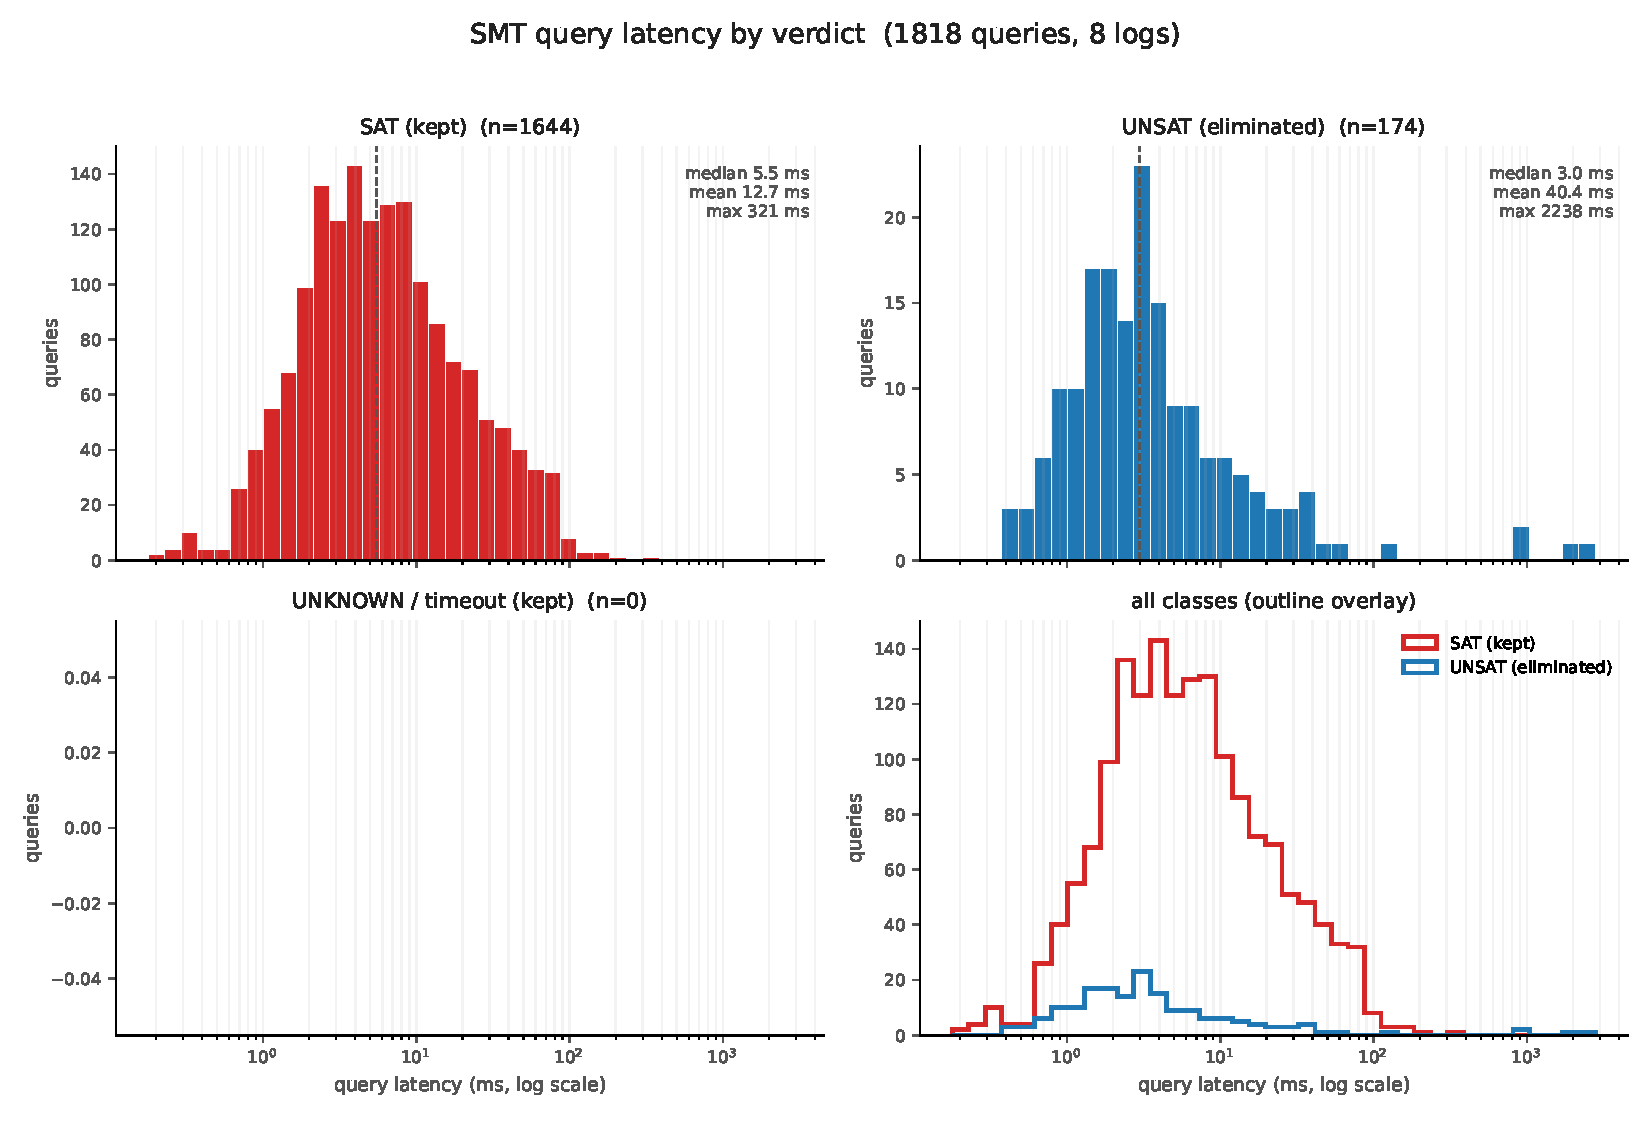
\includegraphics[width=0.92\textwidth]{smt_latencies.pdf}
\caption{SMT query latency by verdict class (1{,}818 queries over eight
runs of zlib's \texttt{deflate} module: signed and unsigned
specifications $\times$ O1 and O3 $\times$ light and heavy tiers, the two
tiers yielding identical verdict sets; unbounded per-query budget). Proofs are
\emph{cheaper} than refutations at the median (\textsc{unsat} 3.0\,ms vs.\
\textsc{sat} 5.5\,ms); the expense lives entirely in a thin tail
(\textsc{unsat} max 2{,}238\,ms). This is the distribution that makes the
timeout dial of Table~\ref{tab:dial} effective: a tight budget truncates
the tail while retaining nearly every proof. Note that this workload class
is the easy end of the spectrum --- the OpenSSL queries discussed below
sit three decades to the right.}
\Description{Four panels of histograms of SMT query latency on a
logarithmic x-axis. The SAT panel shows 1644 queries centered near 5
milliseconds; the UNSAT panel shows 174 queries centered near 3
milliseconds with a small tail beyond one second; the UNKNOWN panel is
empty; the fourth panel overlays the two distributions.}
\label{fig:latency}
\end{figure*}
\begin{table}
\caption{The timeout dial (zlib deflate, unsigned, O1: 457 queries,
8 workers, x86). \textsc{unsat} yield saturates three decades before
the default budget; wall-clock is flat throughout.}
\label{tab:dial}
\small
\begin{tabular}{rrrrr}
\toprule
Budget & \textsc{unsat} & \textsc{sat} & \textsc{unknown} & Wall\\
\midrule
1\,ms & 16 & 66 & 375 & 3.95\,s\\
10\,ms & 43 & 319 & 95 & 4.11\,s\\
100\,ms & \textbf{50} & 405 & 2 & 4.21\,s\\
3\,s & 52 & 405 & 0 & 4.25\,s\\
10\,s & 52 & 405 & 0 & 4.32\,s\\
\bottomrule
\end{tabular}
\end{table}
\paragraph{Compile cost.}
Whole-library zlib costs 131--207\,s of solver stage (about 100--160\,ms
per trap of wall time at 5 processes $\times$ 8 threads) against a 6\,s
unsanitized compile. Per-trap jobs are share-nothing and embarrassingly
parallel; the thread dial of Figure~\ref{fig:matrix} gives $3.8\times$
at 8 workers and plateaus at $4.05\times$ by 16 (Amdahl: serial
discovery plus the slow-query tail).
\paragraph{The dial.}
Table~\ref{tab:dial} is the central cost result: \pct{96} of the provable
facts (50 of 52) survive a \emph{100\,ms} per-query budget, and the
verdict set is fully saturated by 3\,s --- so the default budgets used
throughout this paper sit on a plateau where proof yield is
budget-insensitive. Median \textsc{unsat} latency on this workload is
$\sim$3\,ms; the budget exists for the tail.
Figure~\ref{fig:latency} shows why the dial is so cheap to turn: across
1{,}818 real queries the proofs we want are \emph{faster} than the
refutations we discard, and the cost sits in a thin high-latency tail that
a per-query budget removes almost losslessly.
\begin{figure}
\centering
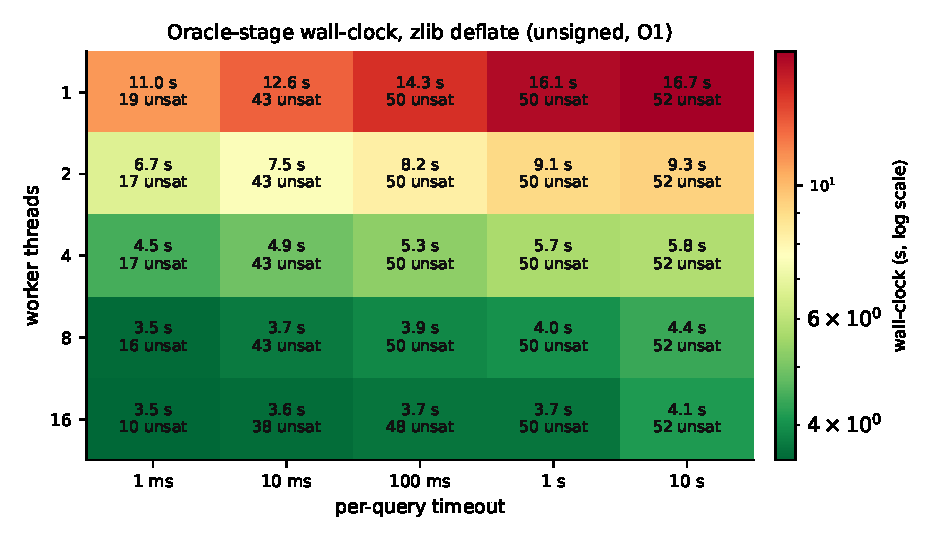
\includegraphics[width=\columnwidth]{dial_matrix.pdf}
\caption{The two dials compose. Oracle-stage wall-clock (median of 3
pinned runs) for the Table~\ref{tab:dial} workload over worker threads
$\times$ per-query timeout; each cell also shows its \textsc{unsat}
yield. Proof yield is set by the timeout alone (every column agrees
with Table~\ref{tab:dial} to the proof, row-independent down to 10\,ms);
wall-clock is set mostly by threads. Serially, the timeout dial is worth
$1.5\times$ (16.7\,s $\to$ 11.0\,s); at 8 threads the pool has already
absorbed the tail and the same dial is worth $1.24\times$. Corner to
corner: $4.8\times$. Below 10\,ms at 16 threads the budget begins to
interact with oversubscription --- a wall-clock budget under contention
--- and the yield dips (52 $\to$ 38 proofs), the one region where the
two knobs are not independent.}
\Description{A five-by-five heatmap, rows are 1 to 16 worker threads,
columns are per-query timeouts from 1 millisecond to 10 seconds. Cells
are colored from red for slow to green for fast on a log scale and
annotated with wall-clock seconds and UNSAT counts. Wall-clock falls
from 16.7 seconds at one thread to about 4 seconds at 8 and 16 threads;
UNSAT counts rise left to right from 16 to 52 in every row.}
\label{fig:matrix}
\end{figure}
\paragraph{The far end of the dial.}
OpenSSL's SHA-256, compiled with aggressive inlining, is the counterpoint:
each of its 2225 unsigned-spec queries carries the false-edges of up to
$\sim$200 \emph{preceding} overflow checks as dominating context. At
0.3--5\,s budgets the pass proves \emph{nothing} (all queries pinned at
the cap; identical for light and heavy tiers); at 30\,s, 43 proofs
appear; an uncapped historical run found 125. The budget curve
$0\,@\,1\text{s} \rightarrow 0\,@\,5\text{s} \rightarrow 43\,@\,30\text{s}
\rightarrow 125\,@\,\infty$ is monotone and tier-invariant: query hardness
here scales with inlined guard-chain depth, and the same knob that makes
zlib effectively free spans five orders of magnitude on real code. The
practical reading is favorable: an \emph{online} deployment at
millisecond budgets gets \pct{96} of zlib-class proofs and silently,
soundly skips OpenSSL-class queries (\textsc{unknown} keeps the check);
an offline audit turns the dial up.
%% =====================================================================
\section{Future Work}
\label{sec:future}
In this paper we targeted sanitizer removal as a consequential
optimization; super-analysis, however, is not limited to this
application. A compiler could host a general super-analysis module
following a simple recipe: wherever the compiler's conventional
range and dataflow heuristics fail, formulate the question as an SMT
decision problem and ask for an answer. Such a compiler would be very
slow; a faster alternative is to invoke the expensive super-analyzer only
inside recognized hot loops.
Verification-aware languages carry assertions, loop invariants, and
post-conditions that have already been proven at the source level, and
some of them reach LLVM IR through conventional toolchains: Verus is
Rust, and so compiles through \texttt{rustc} to LLVM IR directly, while
Dafny~\cite{leino2010dafny} can reach LLVM IR through its (partial,
unsupported) C++ backend. A super-analyzer could use these proven
assertions as an additional rich fact source.
%% =====================================================================
\section{Conclusion}
\label{sec:conclusion}
Super-analysis occupies a deliberately asymmetric point between conventional heuristic-based
optimization and superoptimization: use a solver where analysis precision is the
bottleneck, and conventional machinery everywhere else. Instantiated in
\tool{}, the paradigm proves up to \pct{13.6} of sanitizer checks dead
across real C libraries and yield hot-loop proofs for kernels ---
every deletion certified by an unsat core, audited for vacuity, and
validated by byte-identical output --- and, where proofs gate
transformations, converts them into up to $4.16\times$ speedups on two
ISAs. The unsat cores certify the
paradigm's premise --- the missing reasoning is conjunctive across
analysis domains. Speedup results are proven to be robust by running experiments on inputs of different sizes. Super-analysis has been proven to be an online tool, demonstrated by the fact that \tool{}'s SMT latency can be reduced up to $4.8\times$ by parallelization and strict timeout setting.
%% =====================================================================
\begin{acks}
%% Anonymized for review.
\end{acks}
\section*{Ethics and Privacy Statement}
This work removes only program checks that are formally proven unreachable,
preserving all safety guarantees of the original binaries; every
elimination carries a machine-checkable certificate and our tool refuses
proofs it cannot audit. A dual-use consideration is that reachability
analysis of safety checks could, in principle, help locate reachable
(buggy) checks; this information is equally available to standard fuzzing
and static analysis, and our tool neither exploits nor reports it beyond
keeping such checks intact. No human subjects or personal data are
involved.
\bibliographystyle{ACM-Reference-Format}
\bibliography{odessy}
%% =====================================================================
\appendix
\section{Reproducibility Summary}
Verdicts, output IR, and logs are invariant in \texttt{threads=N} by the
FactGate construction (\S\ref{sec:system-facts}); the acceptance test is a
\texttt{diff} of \texttt{threads=1} vs.\ \texttt{threads=8} outputs.
Hardware is specified to the CloudLab node type (\texttt{c220g2}), whose
full specification is published; all timed runs disable turbo and pin to
one socket; medians over shuffled interleaved repetitions are primary
throughout. An artifact with the pass, benchmarks, harnesses, and raw
per-repetition CSVs is prepared for submission.
\section{Complete Runtime Results}
\label{sec:app-full}
Table~\ref{tab:speedups-full} is the unabridged version of
Table~\ref{tab:speedups}: every benchmark with a runtime experiment,
sorted by speedup. The rows below zstd
compression are the ones that carry the dose--response argument of
\S\ref{sec:results-perf} --- flat where proofs land cold, negative where
non-unlocking elimination loses the re-optimization lottery.
Benchmarks with no runtime experiment split into two further tables.
Table~\ref{tab:frontier} is the \emph{frontier}: benchmarks with a
real, measured ceiling that the current fact sources leave entirely (or
almost entirely) unrecovered --- each row prices a residue class of
\S\ref{sec:future}, and together they show the residue is not cheap
checks nobody cares about. Table~\ref{tab:static-only} collects the
static-only runs, where no ceiling exists to recover --- by measurement
(a $\leq$noise gap), by construction (OpenSSL's signed spec emits no
checks), or because the specification that emits the checks is
dynamically un-runnable in trap mode
(\S\ref{sec:results-static}). Ceilings are checked-vs-unchecked
for native kernels and measured sanitizer overhead for C libraries.
\begin{table*}
\caption{All benchmarks and their runtime results. ``Elim'' is proven
trap edges at the final encoder and full fact tier; speedups are medians
of $\geq$21 shuffled interleaved repetitions, oracle vs.\ the double-O3
control, behind a byte-identical-output gate. Ceilings are per-platform.}
\label{tab:speedups-full}
\small
\begin{tabular}{llrllrrl}
\toprule
Benchmark & Lang & Elim & Platform & Speedup & Ceiling & Recov. & Unlock / note\\
\midrule
\multicolumn{8}{l}{\emph{Proofs that paid}}\\
gemm (stdlib) & Julia & 16 & M-series & $4.16\times$ & $4.19\times$ & 99.8\% & vec+unroll, via \texttt{@inbounds}\\
gemm (stdlib) & Julia & 16 & x86 & $3.59\times$ & $3.97\times$ & 96.4\% & vec+unroll, via \texttt{@inbounds}\\
sha256 & Swift & 7 & x86 & $+8.8$\% & 9.0\% & 98\% & unroll\\
sha256 & Swift & 7 & M-series & $+6.9$\% & 2.8\% & --- & unroll; exceeds checked-vs-unchecked gap\\
sha256 & Julia & 10 & M-series & $+6.9$\% & $-7.9$\% & --- & \texttt{@inbounds} on 6 of 12 sites; lottery-paid (no arm64 ceiling)\\
adler32 & Swift & 1 & x86 & $+3.7$\% & 11.6\% & 32\% & DO16 unrolled group\\
zstd comp.\ (signed) & C & 6 & x86 & $+2.3$\% & 1.2\% & --- & hot group; exceeds overhead ceiling\\
sha1 & Swift & 7 & M-series & $+2.1$\% & 7.6\% & 27\% & unroll (base encoder: $+6.4/{+}7.3$\%)\\
\midrule
\multicolumn{8}{l}{\emph{Proofs that did not pay}}\\
zlib decomp.\ (signed) & C & 113 & x86 & $+0.3$\% & 1.1\% & $\approx$0 & none (cold)\\
zstd decomp.\ (signed) & C & 6 & x86 & $+0.0$\% & 9.0\% & $\approx$0 & none (cold)\\
utf8 validator & Swift & 2 & x86 & $+0.00$\% & 7.5\% & 0 & none; off hot path\\
zlib comp.\ (both spec) & C & 145 & x86 & $+0.1$\% & 5.4\% & $\approx$0 & none (cold); 3 sizes, 3 tiers\\
lz4 comp. & C & 193$^{\P}$ & x86 & $\approx0$\% & 2.0\% & $\approx$0 & none (cold)\\
CryptoSwift (library) & Swift & 183 & x86 & $\pm0.3$\% & 10.4\%$^{c}$ & $\approx$0 & none; cold API surface\\
CryptoSwift (library) & Swift & 215 & M-series & $-0.4$\% & $-0.7$\%$^{c}$ & --- & none; 10\,s budget dose; no ceiling on M-series\\
md5 & Swift & 5 & M-series & $+0.2$\% & $-1.4$\% & --- & none; no ceiling on M-series\\
adler32 & Swift & 1 & M-series & $-1.5$\% & 8.9\% & $<0$ & none; relottery\\
md5 & Swift & 1 & x86 & $-1.8$\% & 6.0\% & $<0$ & none; relottery\\
utf8 validator & Swift & 2 & M-series & $-2.9$\% & $-0.8$\% & --- & none; no ceiling on M-series\\
filt (DSP.jl port) & Julia & 6 & M-series & $-3.7$\% & $-1.6$\% & --- & \texttt{@inbounds} on 2 of 9 sites; no ceiling on arm64\\
sha1 & Swift & 2 & x86 & $-5.0$\% ($\times4$) & 4.7\% & $<0$ & none; replicated relottery\\
\bottomrule
\end{tabular}\\
\raggedright\footnotesize $^{\P}$Marginal over the double-O3 control:
\tool{} removes 1027 of 3403 traps, the control removes 834.
$^{c}$Honest ceiling after removing the \texttt{-O}-vs-sandwich
pipeline gap: on x86, 8.1 points of the raw \pct{19.6}; on M-series the
raw gap is only \pct{1.1} and the pipeline accounts for all of it
(sandwich vs.\ \texttt{-Ounchecked}: \pct{-0.7}, 15 interleaved runs).\par
\end{table*}
\begin{table}
\caption{The frontier: benchmarks with a measured, unrecovered
checked-vs-unchecked ceiling and no (or unusably few) proofs at the
current fact sources. Each ceiling prices a residue class of
\S\ref{sec:future}.}
\label{tab:frontier}
\small
\begin{tabular}{llrlrl}
\toprule
Benchmark & Lang & Elim & Platform & Ceiling & Residue\\
\midrule
nbody & Swift & 0 & M \& x86 & $+410/411$\% & (b), call-carried\\
filt (DSP.jl) & Julia & 4/19 & x86 & 58.3\% & partial edge set\\
base64 & Swift & 0 & x86 & 56.8\% & (d)$+$(b)\\
lz77 & Julia & 0 & x86 & 326\% & checks are the spec\\
matmul & Julia & 0 & x86 & 14.4\% & checks are the spec\\
sha256 & Julia & 2/16 & x86 & 9.5\% & partial edge set\\
crc32 (zlib port) & Swift & 0 & x86 & 4.6\% & (d)\\
lz77 & Swift & 2 & x86 & 3.3\% & unreached ceiling\\
\bottomrule
\end{tabular}\\
\raggedright\footnotesize Julia sha256/filt: the x86 emission proves
only 2 of 16 and 4 of 19 edges (vs.\ 10 and 6 on M-series, where the
ceiling is $\leq 0$) --- too few to license any hot access. Julia
matmul/lz77 M-series ceilings: \pct{1.7} / \pct{158}.\par
\end{table}
\begin{table}
\caption{Static-only runs: no ceiling exists to recover, by
measurement or by construction.}
\label{tab:static-only}
\small
\begin{tabular}{llrlrl}
\toprule
Benchmark & Lang & Elim & Platform & Ceiling & Why static-only\\
\midrule
OpenSSL sha256 & C & 43 & x86 & 0\%$^{d}$ & asm fast path\\
lz4 decomp. & C & --- & x86 & $+0.2$\% & below noise\\
poly (Horner) & Julia & 1 & both & 0.0\% & no ceiling, either ISA\\
zlib decomp.\ (both spec) & C & --- & x86 & n/a & traps fire; un-runnable\\
zstd comp.\ (unsigned) & C & --- & x86 & n/a & traps fire; un-runnable\\
\bottomrule
\end{tabular}\\
\raggedright\footnotesize $^{d}$Exactly zero by construction: under the
signed specification OpenSSL's SHA-256 emits no checks at all. The two
un-runnable rows have no measurable ceiling of any kind: the sanitized
binary executes an intentional-wraparound trap on its first blocks, so
a checked-vs-unchecked comparison cannot be run --- their runnable-spec
counterparts (zlib decomp.\ signed \pct{1.1}, zstd comp.\ signed
\pct{1.2}) appear in Table~\ref{tab:speedups-full}.\par
\end{table}
\begin{figure*}
\centering
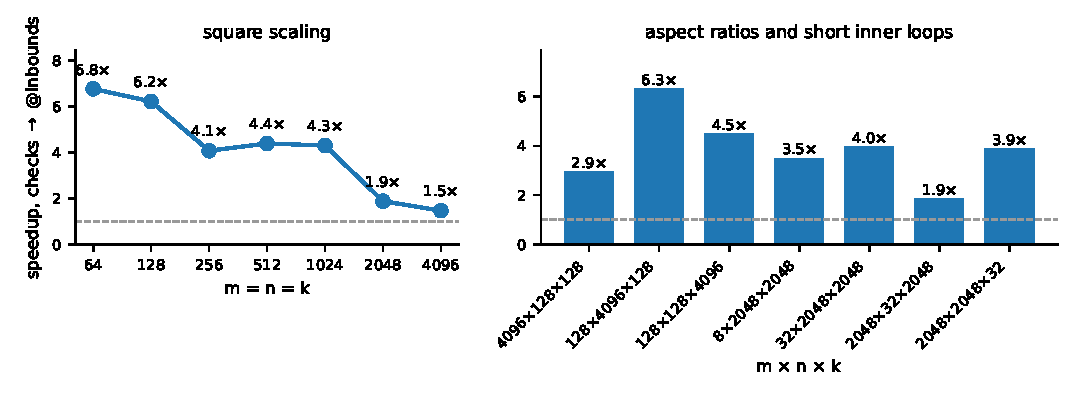
\includegraphics[width=0.92\textwidth]{gemm_sweep.pdf}
\caption{GEMM speedup of the proof-licensed build (all four accesses
\texttt{@inbounds}, which with 16-of-16 edges proven is
source-identical to \tool{}'s arm) over the all-checks baseline, as a
function of the problem shape ($C = m{\times}n$, $A = m{\times}k$,
$B = k{\times}n$; Xeon c220g2, medians of 11 rotated repetitions,
bitwise-equal outputs at every shape). \emph{Left:} square scaling.
\emph{Right:} aspect ratios at roughly constant work and short inner
loops. The gain is present at every shape ($1.5\times$--$6.8\times$)
and is governed by the memory regime of the inner loop over $m$, which
the eliminated checks unblock for vectorization: while its column
working set is cache-resident the unlock pays $4$--$7\times$; at
$m \geq 2048$ (the $2048^3$ and $4096^3$ points and the $m{=}2048$
bars) the loop streams 16--32\,KB columns from memory and bandwidth,
not checks, becomes the limiter --- the floor descends from
$1.9\times$ to $1.5\times$ at $4096^3$ (137\,GFLOP, medians of 5) and
does not approach $1\times$.}
\Description{Two panels. Left, a line chart of speedup versus square
matrix dimension from 64 to 4096 on a log axis: about 6.8x and 6.2x at
64 and 128, about 4.1 to 4.4x from 256 to 1024, 1.9x at 2048, and
1.5x at 4096.
Right, a bar chart of seven non-square shapes with speedups between
1.9x and 6.3x.}
\label{fig:gemm-sweep}
\end{figure*}
\end{document}